% ==============================================================================
% main.tex
% Full Preliminary Design Report — Fuel&Go (Team NextMind, Assignment 02)
% Provisional Option A Target: Exactly 25 Total PDF Pages
% Engine: LuaLaTeX + Biber (IEEE Style) | Custom Class: nextmind-pdr.cls v0.3.2
% ==============================================================================
\documentclass{nextmind-pdr}

\usepackage{csquotes}
\usepackage[backend=biber, style=ieee, sorting=none]{biblatex}
\addbibresource{bib/references.bib}

\setrunningtitle{Fuel\&Go --- Preliminary Design Report}
\setrunningmeta{Team NextMind | Assignment 02}
\setrunningfooter{Fuel\&Go Preliminary Design Report --- Conceptual System Design (\texttt{nextmind-pdr.cls} v0.3.3)}

% Clean spacing calibration for exact 25-page Option A budget (preserves 10pt body font)
\geometry{top=15mm, bottom=14.5mm, left=16.5mm, right=16.5mm, headsep=4.5mm, footskip=7.5mm}
\setstretch{1.01}
\setlength{\parskip}{1.5pt}
\renewcommand{\arraystretch}{1.04}
\setlength{\floatsep}{5pt plus 1pt minus 1pt}
\setlength{\textfloatsep}{6pt plus 1pt minus 1pt}
\setlength{\intextsep}{5pt plus 1pt minus 1pt}
\setlength{\bibitemsep}{1pt}
\renewcommand*{\bibfont}{\footnotesize}

\begin{document}

% ==============================================================================
% FRONT MATTER (Pages 1–3: Cover, Document Control & Executive Summary, ToC)
% ==============================================================================
% ==============================================================================
% front/cover.tex
% Front A — Cover Page (1.0 page indicative)
% ==============================================================================
\thispagestyle{empty}

\begin{tikzpicture}[remember picture, overlay]
  \fill[fgCream] (current page.south west) rectangle (current page.north east);
  \fill[fgPaleSage] ($(current page.north west)+(0,-68mm)$) -- (current page.north east) --
                    ($(current page.north east)+(0,-112mm)$) -- ($(current page.north west)+(0,-88mm)$) -- cycle;
  \fill[fgTeal] (current page.north west) rectangle ($(current page.north east)+(0,-7mm)$);
  \fill[fgAmber] ($(current page.north west)+(0,-7mm)$) rectangle ($(current page.north east)+(0,-8.6mm)$);
  \fill[fgTeal] (current page.south west) rectangle ($(current page.north west)+(6mm,-8.6mm)$);
  \fill[fgSoftCream] (current page.south west) rectangle ($(current page.south east)+(0,30mm)$);
  \draw[fgAmber, line width=1pt] ($(current page.south west)+(6mm,30mm)$) -- ($(current page.south east)+(0,30mm)$);
\end{tikzpicture}

\vspace*{2mm}

\noindent
\begin{tabularx}{\linewidth}{@{}m{26mm} L@{}}
  
\includegraphics[width=22mm]{figures/fuelandgo_logo.png} &
  \kicker{Preliminary Design Report --- Conceptual System Design}\par
  \vspace{2pt}
  {\small\color{fgTeal}\textbf{Assignment 02} \quad|\quad Custom Document Class \texttt{nextmind-pdr.cls}}
\end{tabularx}

\vspace{5mm}

{\raggedright\hyphenpenalty=10000\exhyphenpenalty=10000
  {\headingfont\fontsize{24pt}{28pt}\selectfont\bfseries\color{fgEspresso}
    Fuel\&Go: Preliminary Design Report for a Unified Smart Fueling and EV Charging Platform\par}
  \vspace{3mm}
  {\large\color{fgTeal}\textbf{Business Context, System Architecture, Integration Boundaries, Safety Controls, and Verification Plan}\par}
  \vspace{1.5mm}
  {\normalsize\color{fgOliveDark} Unified Dual-Energy Core Scope (\texttt{FR-01}--\texttt{FR-06b}, \texttt{NFR-01a}--\texttt{NFR-07b}) \quad|\quad Conceptual System Design\par}
}

\vspace{4mm}
\noindent\textcolor{fgAmber}{\rule{48mm}{2pt}}
\vspace{4mm}

\begin{center}
  % ==============================================================================
% figures/cover_illustration.tex
% Bespoke TikZ Vector Illustration for Fuel&Go Editorial Cover (Page 1)
% Combines Fuel Forecourt Canopy/Dispenser, EV Fast-Charger, Sweeping Road,
% Energy-Flow Paths, and Droplet Geometry Echoes.
% ==============================================================================
\begin{tikzpicture}[x=1mm, y=1mm]
  % Soft architectural horizon card
  \fill[fgWhite, rounded corners=5pt] (0,0) rectangle (168,84);
  \draw[fgRuleGray, line width=0.8pt, rounded corners=5pt] (0,0) rectangle (168,84);

  % Subtle sky / terrain bands inside illustration
  \fill[fgSoftCream, rounded corners=4pt] (1,34) rectangle (167,83);
  \fill[fgPaleSage!70] (1,1) rectangle (167,35);

  % Subtle droplet geometry echo in background center
  \begin{scope}[shift={(84,55)}, opacity=0.14]
    \fill[fgTeal] (0,21) .. controls (10,9) and (15,0) .. (15,-7)
      arc (0:-180:15) .. controls (-15,0) and (-10,9) .. (0,21) -- cycle;
  \end{scope}

  % Sweeping curved road connecting Fuel Forecourt (left) & EV Station (right)
  \draw[fgEspresso!85, line width=11mm, line cap=round]
    (12,15) .. controls (54,6) and (66,38) .. (84,34)
            .. controls (102,30) and (116,10) .. (156,19);
  \draw[fgCream, dashed, line width=0.9pt, dash pattern=on 4mm off 3mm]
    (12,15) .. controls (54,6) and (66,38) .. (84,34)
            .. controls (102,30) and (116,10) .. (156,19);

  % --------------------------------------------------------------------------
  % LEFT: Fuel Forecourt Canopy & Dispenser (Terracotta + Amber)
  % --------------------------------------------------------------------------
  % Canopy roof
  \fill[fgTerracotta, rounded corners=2pt] (12,62) rectangle (54,68);
  \fill[fgAmber] (12,61) rectangle (54,62.4);
  % Canopy pillars
  \fill[fgEspresso!75] (18,34) rectangle (20.5,61);
  \fill[fgEspresso!75] (46,34) rectangle (48.5,61);
  % Dispenser island
  \fill[fgRuleGray, rounded corners=1.5pt] (26,33) rectangle (41,36);
  % Dispenser body
  \fill[fgWhite, rounded corners=1.5pt] (29,36) rectangle (38,53);
  \draw[fgTerracotta, line width=1pt, rounded corners=1.5pt] (29,36) rectangle (38,53);
  \fill[fgTerraTint] (30.5,46) rectangle (36.5,51);
  \draw[fgTerracotta, line width=0.6pt] (30.5,46) rectangle (36.5,51);
  % Nozzle & hose
  \draw[fgEspresso, line width=1.1pt] (38,49) .. controls (42,49) and (42,40) .. (38.5,40);
  \fill[fgTerracotta] (39.5,47.5) rectangle (41.5,50.5);
  % Label pill
  \node[rectangle, rounded corners=2pt, fill=fgTerraTint, draw=fgTerracotta, line width=0.7pt,
        font=\footnotesize\bfseries, text=fgTerracotta, inner xsep=5pt, inner ysep=2pt]
        at (33,74) {Fuel Forecourt};

  % --------------------------------------------------------------------------
  % RIGHT: EV Fast-Charging Station (Eco Green + Teal)
  % --------------------------------------------------------------------------
  % Station canopy arc
  \fill[fgEcoGreen, rounded corners=2pt] (114,62) rectangle (156,68);
  \fill[fgTeal] (114,61) rectangle (156,62.4);
  % Pillar
  \fill[fgEspresso!75] (148,34) rectangle (150.5,61);
  % EV Charger pedestal
  \fill[fgEcoTint, rounded corners=1.5pt] (124,33) rectangle (140,36);
  \fill[fgWhite, rounded corners=2pt] (127,36) rectangle (137,55);
  \draw[fgEcoGreen, line width=1pt, rounded corners=2pt] (127,36) rectangle (137,55);
  \fill[fgEcoTint] (128.8,47) rectangle (135.2,52.5);
  \draw[fgEcoGreen, line width=0.6pt] (128.8,47) rectangle (135.2,52.5);
  % Lightning bolt inside EV pedestal
  \fill[fgEcoGreen] (132.4,51.7) -- (130.6,49.4) -- (131.9,49.4) -- (131.5,47.6) -- (133.5,49.9) -- (132.1,49.9) -- cycle;
  % Charging cable
  \draw[fgTeal, line width=1.1pt] (127,48) .. controls (122.5,48) and (122.5,39) .. (126.5,39);
  % Label pill
  \node[rectangle, rounded corners=2pt, fill=fgEcoTint, draw=fgEcoGreen, line width=0.7pt,
        font=\footnotesize\bfseries, text=fgEcoGreen, inner xsep=5pt, inner ysep=2pt]
        at (135,74) {EV Fast-Charging};

  % --------------------------------------------------------------------------
  % CENTER: Unified Fuel&Go Core Hub + Dual Energy-Flow Paths
  % --------------------------------------------------------------------------
  \node[circle, fill=fgTeal, draw=fgAmber, line width=1.4pt, minimum size=19mm,
        font=\footnotesize\bfseries, text=fgWhite, align=center] (hub) at (84,54) {Fuel\&Go\\Core};

  % Fuel energy-flow arc (solid terracotta + arrow)
  \draw[fgTerracotta, line width=1.3pt, -{Stealth[length=2.4mm]}]
    (43,51) .. controls (56,57) and (64,57) .. (hub.west);
  % EV energy-flow arc (solid eco green + arrow)
  \draw[fgEcoGreen, line width=1.3pt, -{Stealth[length=2.4mm]}]
    (125,51) .. controls (112,57) and (104,57) .. (hub.east);

  % Subtle caption bar inside bottom of illustration
  \node[font=\footnotesize\bfseries, text=fgTeal] at (84,6.5)
    {Single Driver Journey across ICE Refueling \& EV Charging Networks};
\end{tikzpicture}

\end{center}

\vspace{4mm}

\noindent
\begin{tcolorbox}[
  enhanced,
  colback=fgWhite,
  colframe=fgRuleGray,
  borderline west={4pt}{0pt}{fgOlive},
  boxrule=0.6pt,
  arc=3pt,
  left=10pt, right=10pt, top=7pt, bottom=7pt
]
  \begin{tabularx}{\linewidth}{@{}L L@{}}
    {\footnotesize\textcolor{fgTextAmber}{\textbf{PREPARED BY}}}\par
    \vspace{2pt}
    {\headingfont\large\bfseries\color{fgEspresso} Team NextMind}\par
    {\small\color{fgEspresso} Maria Mnasra \quad\&\quad Basmala Jamal}\par
    {\footnotesize\color{fgEspresso!80} Assignment 02 --- Department of Management, Bar-Ilan University (November 2026).}
    &
    {\footnotesize\textcolor{fgTextAmber}{\textbf{DOCUMENT GOVERNANCE STATUS}}}\par
    \vspace{2pt}
    {\small\color{fgTeal}\textbf{Conceptual System Design}}\par
    {\footnotesize\color{fgEspresso!80} Working visual design direction applied; formal partner review and final scope sign-off remain pending. All runtime targets and delivery estimates are preliminary proposals.}
  \end{tabularx}
\end{tcolorbox}

\vfill

\noindent
\begin{tabularx}{\linewidth}{@{}L r@{}}
  {\footnotesize\color{fgEspresso!80}
    \textbf{Epistemic Notice:} This report documents a conceptual system design. No production deployment, partner commercial agreements, or field measurements are claimed.
  } &
  {\footnotesize\color{fgTeal}\textbf{v1.0 (Working)}}
\end{tabularx}

\clearpage


% ==============================================================================
% front/executive_summary.tex
% Front B — Document Control, Executive Summary & Audience Framing (1.0 page)
% ==============================================================================
{\headingfont\Large\bfseries\color{fgEspresso} Document Control \& Executive Summary}\par
\vspace{-2pt}\noindent\textcolor{fgAmber}{\rule{\linewidth}{1.1pt}}
\vspace{4pt}

\noindent
{\footnotesize
\begin{tabularx}{\linewidth}{@{}P{32mm} L P{30mm} L@{}}
  \toprule
  \rowcolor{fgOlive}
  \fgtableheader{Attribute} & \fgtableheader{Value} & \fgtableheader{Attribute} & \fgtableheader{Value} \\
  \midrule
  \textbf{Document Title} & Fuel\&Go Preliminary Design Report & \textbf{Team / Authors} & Team NextMind (Maria Mnasra, Basmala Jamal) \\
  \rowcolor{fgSoftCream}
  \textbf{Design Status} & Conceptual System Design (Partner Review Pending) & \textbf{Course / Deliverable} & Assignment 02 (25-Page Technical Report) \\
  \textbf{Core Scope} & Unified ICE Fueling \& EV Charging (\texttt{FR-01}--\texttt{FR-06b}) & \textbf{Visual Direction} & Fuel\&Go Presentation Palette (WCAG AA Hardened) \\
  \rowcolor{fgSoftCream}
  \textbf{Build Toolchain} & LuaLaTeX + Biber (IEEE Style) + Python 3 & \textbf{Date / Revision} & November 2026 \quad|\quad Working Release v1.0 \\
  \bottomrule
\end{tabularx}
}

\vspace{3pt}

\subsection*{Executive Summary}
\vspace{-2pt}
Drivers across internal-combustion (ICE), plug-in hybrid (PHEV), and battery-electric (BEV) fleets face a fragmented refueling experience split across brand-locked fuel apps, incompatible EV charging networks, and manual payment counters. Global electric car sales exceeded 17~million in 2024---over 20\% of new car sales worldwide~\cite{iea2025gev}---accelerating the transition toward mixed-energy mobility where drivers and households increasingly operate both liquid-fuel and electric vehicles. \textbf{Fuel\&Go} is proposed as a unified, driver-first mobile platform that consolidates station discovery, remote bay authorization, real-time dispensing/charging telemetry, tokenized contactless payment, and fault recovery into a single cross-operator workflow.

\begin{insightcard}[Core Scope, Architecture \& Safety Highlights]
  \begin{itemize}[leftmargin=12pt, itemsep=1pt, topsep=1pt]
    \item \textbf{Disciplined Core Scope:} Chapters~1--8 specify six core functional domains (\texttt{FR-01}--\texttt{FR-06b}) and seven non-functional requirement families (\texttt{NFR-01a}--\texttt{NFR-07b}). Source-supported extensions (\texttt{EXT-02}--\texttt{EXT-05}) are deferred to Phase~3; unsupported/unapproved items (\texttt{EXT-01}, corporate VAT invoicing, standalone operator dashboard, AI Guidance Assistant) remain excluded from Core scope.
    \item \textbf{Decoupled Integration Architecture:} Fuel\&Go implements four interfaces---Mobile$\leftrightarrow$Backend (REST + WebSocket~\cite{rfc9110,rfc6455}), Backend$\leftrightarrow$EV Operator/Roaming (candidate OCPI~\cite{evroaming2025ocpi}), Backend$\leftrightarrow$Forecourt/POS (candidate IFSF~\cite{ifsf_specs}), and Backend$\leftrightarrow$PSP (tokenized APIs under PCI~DSS~v4.0.1~\cite{pcissc2024pcidss401})---while treating OCPP~\cite{oca2020ocpp201,oca2025ocpp21} and ISO~15118~\cite{iso15118_2_2014,iso15118_20_2022} as external context domains.
    \item \textbf{Cyber-Physical Safety \& Payment Boundaries:} Under \texttt{NFR-06}, physical emergency stops, overfill/vapor cutoffs, and high-voltage EVSE ground-fault relays remain strictly autonomous at the station hardware layer. PSP tokenization narrows the CDE without by itself establishing PCI~DSS compliance.
  \end{itemize}
\end{insightcard}

\textbf{Top Residual Risks \& Go/No-Go Gates:} Four high-priority risks govern progression to implementation: (1)~multi-operator onboarding and proprietary forecourt gateway variability; (2)~ambiguous authorization-timeout states requiring durable reconciliation rather than blind hold voids; (3)~physical QR-sticker tampering; and (4)~jurisdiction-dependent privacy compliance (Israel PPL Amendment~13~\cite{israel1981ppl} vs.\ conditional EU~GDPR~\cite{eu2016gdpr}). Advancement to MVP requires partner scope sign-off, sandbox agreements with at least one forecourt gateway and one EV CPO, and HIL safety/reconciliation gates.

\vspace{2pt}
\subsection*{Audience Framing}
\vspace{-2pt}
This report serves two distinct reader groups while modeling ICE/hybrid and EV drivers strictly as system actors rather than report readers:

\noindent
{\footnotesize
\begin{tabularx}{\linewidth}{@{}P{42mm} L@{}}
  \toprule
  \rowcolor{fgTeal}
  \fgtableheader{Reader Audience} & \fgtableheader{Primary Information Needs Addressed in This Report} \\
  \midrule
  \textbf{Executive Management \& Product/Engineering Decision-Makers} & Commercial framing (business model, revenue mechanisms, cost drivers, feasibility constraints), disciplined scope governance, weighted architectural trade-offs, residual cyber-physical risk visibility, and a phased product delivery roadmap with explicit go/no-go gates. \\
  \rowcolor{fgSoftCream}
  \textbf{Course Lecturer \& Academic Evaluators} & Compliance with Assignment~02 engineering and typesetting mandates: custom \texttt{nextmind-pdr.cls} template, deterministic LuaLaTeX + Biber IEEE bibliography, reproducible Python figures, zero-fabrication epistemic tagging, and transparent separation of conceptual product verification from actual report QA. \\
  \bottomrule
\end{tabularx}
}

\clearpage


% Compact Table of Contents (Page 3 — fits cleanly on 1 page)
{\headingfont\Large\bfseries\color{fgEspresso} Table of Contents}\par
\vspace{-2pt}\noindent\textcolor{fgAmber}{\rule{\linewidth}{1.1pt}}
\vspace{2pt}
{\small\setstretch{0.96}
\makeatletter
\@starttoc{toc}
\makeatother
}

\clearpage

% ==============================================================================
% BODY CHAPTERS 1–9 (Continuous Flow — No Forced Blank Pages)
% ==============================================================================
% ==============================================================================
% Chapter 1: Introduction, Business Motivation & Scope Boundaries
% Indicative Space Budget: ~1.5 pages
% Status: Draft — Prepared by Research; Pending Partner Review
% ==============================================================================

\fgchapter{01}{Chapter 01 --- Scope \& Framing}{Introduction, Business Motivation \& Scope Boundaries}{Operational pain points, design governance, and core vs.\ roadmap boundaries}{sec:intro}

\subsection{Operational Problem and Business Motivation}
\label{sec:intro-motivation}

Drivers refueling internal-combustion engine (ICE) or hybrid vehicles and drivers charging battery electric vehicles (BEVs) currently navigate a fragmented digital landscape. As documented in the original Fuel\&Go product presentation (\texttt{Fuel\&Go Whole Tasks.pptx}, Slide~2), everyday station visits suffer from five recurring pain points: physical queuing at forecourts, switching between pumps and indoor payment counters, maintaining separate brand-specific mobile applications for different fuel companies, accidental selection of an incompatible fuel grade, and uncertainty regarding real-time electric vehicle (EV) charger availability.

Global market trajectories reinforce the structural need for dual-energy station interfaces. According to the International Energy Agency (IEA) \emph{Global EV Outlook 2025}~\cite{iea2025gev}, global electric car sales (BEV and plug-in hybrid) exceeded 17~million vehicles in 2024---representing more than 25\% year-over-year growth and more than 20\% of all new cars sold worldwide. As public charging expands alongside legacy liquid-fuel infrastructure, drivers increasingly rely on public chargers for inter-city travel and where residential parking lacks dedicated charging access~\cite{iea2025gev}. In Israel---the target deployment jurisdiction referenced in the original Fuel\&Go presentation (Slides~2, 8, and 30; formal jurisdiction confirmation remains pending partner sign-off)---drivers encounter separate mobile applications for fuel chains (such as Paz \texttt{yellow}~\cite{paz2025yellow}) and dedicated EV charging networks (such as EV-Edge~\cite{evedge2025app} and Afcon EV's \texttt{ON}~\cite{afconev2025on}), while navigation applications such as Waze~\cite{waze2025help,waze2025gas} focus on route discovery and community price reporting rather than end-to-end session activation or payment settlement. \emph{Note on local market data}: Official primary-source datasets from the Israel Central Bureau of Statistics (CBS) for 2024--2025 Israeli EV market share have not been directly inspected; unverified secondary press figures are therefore excluded from empirical claims in this report.

\textbf{Fuel\&Go} is conceptualized as a unified mobile refueling and EV charging platform enabling ICE, hybrid, and EV drivers to discover compatible stations, authorize fuel dispensers or EV chargers remotely, monitor live energy delivery, and complete tokenized contactless payments within a single cohesive workflow (\texttt{PRD.md}, Sec.~2; Presentation Slides~1--3).

\subsection{Report Framing and Unresolved Design Decisions}
\label{sec:intro-framing}

This document serves as the \emph{Conceptual System Design} and working \emph{Preliminary Design Report (PDR)} for Fuel\&Go. No runtime software, hardware integration, or payment gateway certification has been implemented or field-tested; all architectural and verification descriptions represent \emph{Proposed Core Interfaces} and \emph{Planned Verification} activities.

Several substantive scope and engineering decisions remain open pending formal stakeholder and engineering sign-off:
\begin{itemize}[leftmargin=1.4em, itemsep=2pt]
  \item \textbf{Deployment Jurisdiction \& Regulatory Scope}: Israel is adopted as the working launch jurisdiction per the original product presentation, subject to formal partner confirmation before locking statutory privacy and payment compliance obligations.
  \item \textbf{Report Title \& Decision Audience}: The working PDR framing and optional secondary management audience (executive and product/engineering decision-makers alongside academic evaluators) remain provisional pending final review.
  \item \textbf{Extension Scope \& Provisional Targets}: Disputed product extensions (\texttt{EXT-01}--\texttt{EXT-05}), the presentation's AI Guidance Assistant, and unbacked numeric non-functional performance targets remain explicitly quarantined or marked provisional pending engineering sign-off.
\end{itemize}

\subsection{Core Scope vs.\ Roadmap and Flagged Feature Boundaries}
\label{sec:intro-scope}

The governing product specification (\texttt{PRD.md}, v1.2.0-draft) establishes six core functional capabilities (\texttt{FR-01}--\texttt{FR-06}) as the baseline for this preliminary design. Direct inspection of \texttt{Fuel\&Go Whole Tasks.pptx} (78~slides) surfaced two provenance findings that are documented transparently without silently altering scope:
\begin{enumerate}[leftmargin=1.4em, itemsep=2pt]
  \item \textbf{AI Guidance Assistant Conflict}: Slides~3 and 40 list an \emph{AI Digital Assistant} under functional features, whereas \texttt{PRD.md} excludes it from \texttt{FR-01}--\texttt{FR-06}. It is therefore quarantined from core architecture pending formal scope resolution.
  \item \textbf{Extension Provenance (\texttt{EXT-01}--\texttt{EXT-05})}: Direct slide extraction confirms that \texttt{EXT-02} (discounts/promotions, Slide~40), \texttt{EXT-03} (fleet management and subscriptions, Slides~4, 30, 40), and \texttt{EXT-04} partial (monthly AI usage/financial summaries, Slide~40) appear in the original presentation as additional features, and \texttt{EXT-05} partial appears as B2B API partner integration (Slides~8, 27). Conversely, \texttt{EXT-01} (convenience-store pre-ordering) and consolidated corporate VAT invoicing are \emph{not} found in the reviewed presentation.
\end{enumerate}

Table~\ref{tab:scope-boundary} summarizes the resulting scope boundary governing Chapters~1--9.

\begin{table}[htbp]
  \centering
  \caption{Fuel\&Go Scope Boundary Matrix: Core Specification vs.\ Roadmap and Quarantined Features.}
  \label{tab:scope-boundary}
  \small
  \begin{tabularx}{\linewidth}{@{}P{28mm} L P{36mm} P{28mm}@{}}
    \toprule
    \rowcolor{fgOlive}
    \fgtableheader{Scope Tier} & \fgtableheader{Capabilities / Items} & \fgtableheader{Source Provenance} & \fgtableheader{Report Treatment} \\
    \midrule
    \textbf{Core Scope} \newline \emph{(Authoritative Spec)} &
    \texttt{FR-01} Account, Auth \& Vehicle Profile; \texttt{FR-02} Unified Station \& Charger Discovery; \texttt{FR-03} Pump/Charger Selection \& Authorization; \texttt{FR-04} Real-Time Telemetry; \texttt{FR-05} Contactless Settlement \& Basic Receipt; \texttt{FR-06} Fault Recovery \& Basic Support. &
    \texttt{PRD.md} Sec.~2.1; Presentation Slides~2--3, 30, 40, 50. &
    Full specification, conceptual architecture, and planned verification (Ch.~1--8). \\
    \midrule
    \textbf{Source-Supported Roadmap} \newline \emph{(Pending Scope Sign-Off)} &
    \texttt{EXT-02} Discounts, coupons \& referral rewards; \texttt{EXT-03} Fleet management \& subscriptions; \texttt{EXT-04} (partial) Monthly AI usage/financial summaries; \texttt{EXT-05} (partial) B2B API partner ecosystem; multilingual UI, route optimization, queue alerts. &
    Presentation Slides~4, 8, 27, 30, 40 (\emph{Additional Features}). &
    Excluded from core architecture depth; staged in Ch.~9 roadmap only. \\
    \midrule
    \textbf{Quarantined / Conflict Flagged} \newline \emph{(Pending Scope Sign-Off)} &
    \textbf{AI Guidance Assistant} (in Slides~3 \& 40, absent from \texttt{PRD.md}); \texttt{EXT-01} C-store food/coffee pre-ordering (not in deck); \texttt{EXT-04} Corporate VAT invoicing (not in deck); \texttt{EXT-05} Standalone operator web dashboard (unverified). &
    Direct OOXML audit of 78-slide deck vs.\ \texttt{PRD.md} v1.2.0-draft. &
    Strictly excluded from core requirements unless formally approved for promotion. \\
    \bottomrule
  \end{tabularx}
\end{table}


\vspace{10pt}
% ==============================================================================
% Chapter 2: Market Context, Business Model, Users & Stakeholders
% Indicative Space Budget: ~2.5 pages
% Status: Draft — Prepared by Research; Pending Partner Review
% ==============================================================================

\fgchapterflow{02}{Chapter 02 --- Market \& Stakeholders}{Market Context, Business Model, Users \& Stakeholders}{Verified EV adoption context, competitor audit, ecosystem roles, and stakeholder matrix}{sec:market-stakeholders}

\subsection{Dual-Energy Market Context and Data Provenance}
\label{sec:market-context}

The commercial rationale for Fuel\&Go rests on the coexistence of legacy liquid-fuel infrastructure and rapidly expanding public EV charging networks. Directly verified 2024 global measurements from the IEA \emph{Global EV Outlook 2025}~\cite{iea2025gev} demonstrate both rapid fleet electrification and regional variation in public charging density:
\begin{itemize}[leftmargin=1.4em, itemsep=2pt]
  \item \textbf{Global Sales Momentum (\texttt{[Sourced Measurement]})}: Electric car sales (BEV and PHEV) exceeded 17~million vehicles globally in 2024---an increase of more than 25\% year-over-year compared to 2023---reaching a sales share of more than 20\% of all new cars sold worldwide~\cite{iea2025gev}.
  \item \textbf{Public Charging Coverage (\texttt{[Sourced Measurement]})}: In 2024, China had \emph{more than 1~public charger for every 10~electric cars} (a reciprocal upper bound of fewer than 10~electric cars per public charger, rather than an exact measured value of~10), whereas the European Union averaged \emph{1~public charger for every 13~electric cars}~\cite{iea2025gev}. Expanding public charging access is particularly important in dense urban areas where apartment housing limits private home charging~\cite{iea2025gev}.
  \item \textbf{Israeli Market Context (\texttt{[Unverified --- Excluded from Empirical Claims]})}: The original Fuel\&Go presentation (Slides~2 and 8) positions Israel as the primary launch market due to rising EV adoption and brand-specific app fragmentation. Because official primary-source tables from the Israel Central Bureau of Statistics (CBS) have not been directly inspected, secondary press summaries of Israeli BEV market share are classified as \emph{unverified} and strictly excluded from empirical claims, calculations, and Figure~\ref{fig:market-context}.
\end{itemize}

% ------------------------------------------------------------------------------
% FIGURE 2.1 HOOK FOR DESIGN AGENT (Reproducible Python Plot #1)
% Source CSV: data/ev_market_summary_verified.csv (iea2025gev rows ONLY;
%             strictly exclude UNVERIFIED_EXCLUDED Israel rows).
% Design Spec (Finding 1):
%   - Do NOT plot vehicle sales (millions) and percentages on a shared numerical axis.
%   - Use separate clearly labeled panels or designed KPI cards.
%   - Preserve "more than" (>) and "on average" (~) qualifiers.
%   - Do NOT plot China's ">1.0 public chargers per 10 electric cars" (<10 EVs/charger)
%     as an exact measured bar of 10.
% Required Provenance Tag in Chart & Caption: [Sourced Measurement] (+ [Calculation] if reciprocal shown)
% ------------------------------------------------------------------------------
\begin{figure}[htbp]
  \centering
  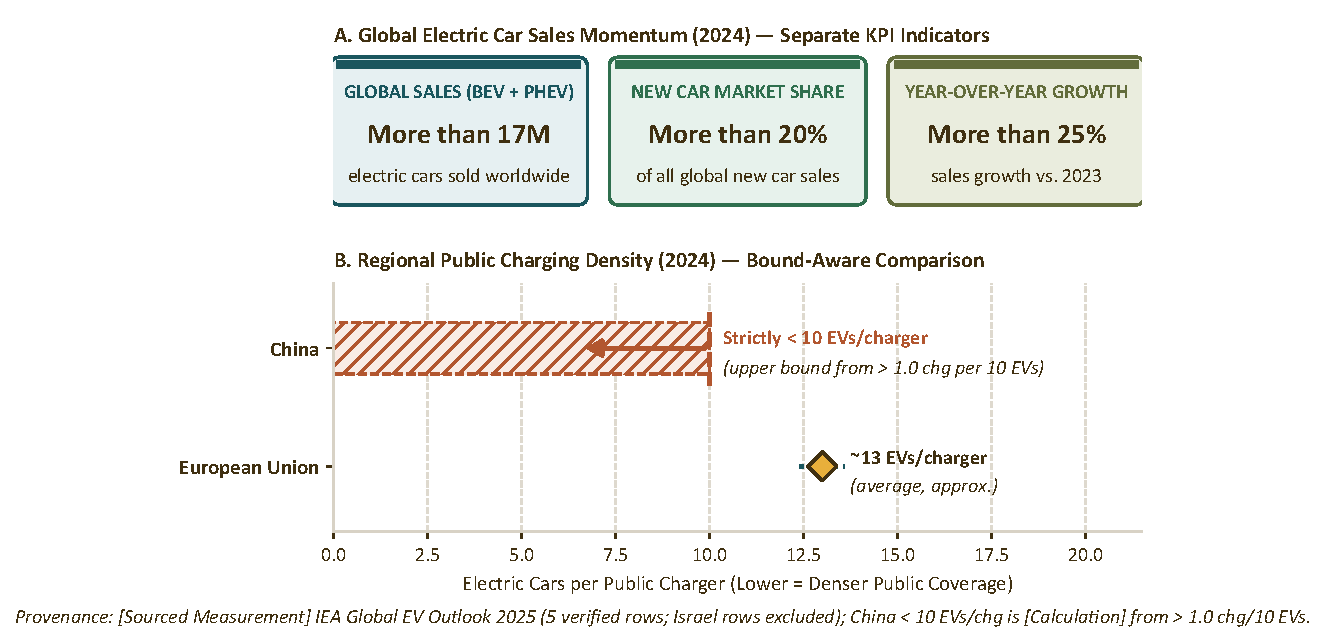
\includegraphics[width=\linewidth]{figures/fig2_1_market_context.pdf}
  \caption{Global EV Adoption and Regional Public Charging Coverage (2024). Separate panels/KPI cards avoid mixing incompatible units and preserve IEA uncertainty qualifiers (``more than'' and ``on average''). \emph{Provenance}: \texttt{[Sourced Measurement]} from IEA \emph{Global EV Outlook 2025}~\cite{iea2025gev} (Executive Summary and Electric Vehicle Charging chapters); China's reciprocal upper bound ($<10$~electric cars per public charger) is a deterministic \texttt{[Calculation]} from IEA's ``more than 1~public charger per 10~electric cars.''}
  \label{fig:market-context}
\end{figure}

\subsection{Competitive Landscape Verification}
\label{sec:competitors}

The original Fuel\&Go presentation (Slides~13, 74, and 75) defines qualitative market tiers (TAM: regular fueling/charging drivers; SAM: drivers at digitally enabled stations; SOM: EV owners and tech-savvy drivers seeking a unified app; Slide~12) and positions Fuel\&Go against navigation apps, fuel-chain apps, and EV-only network apps. Each referenced competitor was verified against official product or help documentation inspected on 2026-11-27:

\begin{itemize}[leftmargin=1.4em, itemsep=2pt]
  \item \textbf{Waze (Navigation-First Indirect Competitor)}~\cite{waze2025help,waze2025gas}: Inspected official Waze Help articles document route-based EV charging station discovery (filtered by plug type and preferred network)~\cite{waze2025help} and community-reported fuel types and gas prices~\cite{waze2025gas}. Within these official guides, Waze's documented scope centers on navigation, discovery, and crowd-sourced pricing rather than remote pump/charger activation, live energy telemetry, or unified payment settlement.
  \item \textbf{Paz \texttt{yellow} App (Brand-Centric Fuel \& Retail Competitor)}~\cite{paz2025yellow}: The inspected official Paz product page documents \texttt{yellow} as a digital wallet and cashback loyalty platform covering fueling at Paz stations, convenience-store purchases, \emph{Paz Charge} EV charging, and partner perks. \emph{Correction vs.\ Slide~74}: Although Slide~74 described \texttt{yellow}'s EV support as limited, current official documentation confirms Paz Charge integration inside \texttt{yellow}. However, the inspected page positions \texttt{yellow} around the Paz and \texttt{yellow} partner ecosystem rather than cross-operator roaming across competing fuel chains and third-party EV Charge Point Operators (CPOs).
  \item \textbf{EV-Edge~\cite{evedge2025app} and Afcon EV \texttt{ON}~\cite{afconev2025on} (EV-Focused Direct Competitors)}: The inspected official EV-Edge public charging network page and Afcon EV \texttt{ON} application page document dedicated Israeli EV charging apps offering station discovery, charger speed/connector filtering, live availability, and mobile payment. Liquid-fuel forecourt dispensing is not part of the documented offering on either inspected page.
\end{itemize}

Fuel\&Go's proposed differentiation (Slide~75) is therefore an \emph{operator-agnostic, dual-energy, end-to-end session flow} spanning discovery, remote activation, live telemetry, and settlement across both liquid-fuel forecourts and EV charging networks.

\subsection{Business Model: Established Ecosystem Roles vs.\ Proposed Mechanisms}
\label{sec:business-model}

To prevent conflating established industry standards with unvalidated commercial claims, Fuel\&Go's business model separates \emph{sourced ecosystem roles} from \emph{proposed monetization mechanisms}:

\begin{enumerate}[leftmargin=1.4em, itemsep=2pt]
  \item \textbf{Established EV Roaming Roles (\texttt{[Sourced Fact]})}: Under the Open Charge Point Interface (OCPI) specification~\cite{evroaming2025ocpi}, the EV charging value chain separates the \textbf{Charge Point Operator (CPO)}---which owns and operates physical chargers and publishes Locations, Tariffs, Sessions, and Charge Detail Records (CDRs)---from the \textbf{e-Mobility Service Provider (eMSP)}---which owns the driver-facing mobile application, authentication Tokens, and driver billing. Standardized CDRs serve as the settlement record between CPO and eMSP~\cite{evroaming2025ocpi}. In this taxonomy, Fuel\&Go operates conceptually as a multi-network eMSP extended with an analogous forecourt integration layer for liquid-fuel operators.
  \item \textbf{Proposed Revenue Mechanisms (\texttt{[Proposed Choice]})}: Building on Presentation Slides~27, 40, and 75, Fuel\&Go's candidate revenue streams are: (a)~per-transaction partner commissions or wholesale-to-retail tariff spreads settled against operator CDRs/forecourt receipts; (b)~B2B API onboarding or integration fees for multi-sided ecosystem partners; and (c)~future subscription tiers for frequent drivers or fleet accounts (\texttt{EXT-03}, roadmap only). No fee percentages, unit margins, partner agreements, or profitability projections are assumed or claimed.
  \item \textbf{Major Cost Drivers \& Feasibility Constraints (\texttt{[Assumption]})}: Operating an aggregator platform entails Payment Service Provider (PSP) processing fees, cloud and real-time telemetry infrastructure, per-operator adapter onboarding and maintenance, security/PCI compliance overhead, customer acquisition cost (CAC), and driver support. Primary commercial feasibility risks include multi-operator onboarding friction and thin retail fuel margins.
\end{enumerate}

\subsection{Report Audience vs.\ System Users and Stakeholders}
\label{sec:users-stakeholders}

Following \texttt{PRD.md} (Sec.~1.3), this report separates \emph{report readers} (academic evaluators and, provisionally, executive and product/engineering decision-makers) from \emph{Fuel\&Go application users}. Within the Fuel\&Go system itself, core end users are \textbf{ICE/Hybrid Vehicle Drivers} and \textbf{EV Drivers} (including accessibility-challenged drivers highlighted on Presentation Slide~4), while external operational stakeholders comprise Fuel Station Operators, EV CPOs, and Payment Service Providers. Fleet managers (\texttt{EXT-03}) and standalone station-operator dashboards (\texttt{EXT-05}) remain outside core scope pending formal scope sign-off. Table~\ref{tab:commercial-stakeholders} consolidates the commercial overview and stakeholder roles.

\begin{table}[htbp]
  \centering
  \caption{Fuel\&Go Commercial Overview, Feasibility Constraints, and Stakeholder Matrix.}
  \label{tab:commercial-stakeholders}
  \small
  \begin{tabularx}{\linewidth}{@{}P{30mm} L P{34mm} P{26mm}@{}}
    \toprule
    \rowcolor{fgOlive}
    \fgtableheader{Dimension / Actor} & \fgtableheader{Role, Mechanism, or Core Concern} & \fgtableheader{Provenance / Basis} & \fgtableheader{Scope / Status} \\
    \midrule
    \textbf{ICE / Hybrid Driver} & Discovers stations with live prices, selects compatible fuel grade, authorizes pump, pays contactlessly, receives digital receipt. & \texttt{PRD.md} Sec.~1.3; Slides~2, 4, 50. & Core End User \\
    \textbf{EV Driver} & Filters compatible connectors/kW ratings, checks live charger status, initiates/stops charging, monitors kWh/SoC, pays contactlessly. & \texttt{PRD.md} Sec.~1.3; Slides~2, 4, 40. & Core End User \\
    \textbf{EV CPO / Roaming Partner} & Operates chargers/CSMS; publishes Locations, Tariffs, Sessions, and CDRs over OCPI~\cite{evroaming2025ocpi} to Fuel\&Go (eMSP role). & \texttt{[Sourced Fact]} OCPI~\cite{evroaming2025ocpi}; Slide~27. & External System Stakeholder \\
    \textbf{Fuel Forecourt Operator} & Operates physical dispensers and forecourt controller/POS gateway; enforces local hardware safety interlocks. & \texttt{PRD.md} Sec.~2.1; IFSF~\cite{ifsf_specs}; Slide~8. & External System Stakeholder \\
    \textbf{Payment Service Provider (PSP)} & Vaults payment credentials, issues surrogate tokens, executes pre-authorization holds, final capture, and hold release. & \texttt{[Sourced Fact]} PCI DSS~\cite{pcissc2024pcidss401}. & External System Stakeholder \\
    \midrule
    \textbf{Revenue Mechanisms} & Candidate per-transaction partner commission, B2B API integration fees, and post-MVP fleet/driver subscriptions. & \texttt{[Proposed Choice]} Slides~27, 40, 75. & Conceptual (No invented financials) \\
    \textbf{Cost Drivers \& Constraints} & PSP fees, cloud/telemetry hosting, operator onboarding/maintenance, security/compliance audits, CAC; margin sensitivity. & \texttt{[Assumption]} Industry context. & Feasibility Constraint \\
    \textbf{Product Success KPIs} & Monthly Active Users (MAU), end-to-end flow completion rate, repeat usage, active ecosystem partners, payment volume. & Presentation Slides~27, 78. & Numeric targets provisional \\
    \bottomrule
  \end{tabularx}
\end{table}


\vspace{10pt}
% ==============================================================================
% Chapter 3: Functional & Non-Functional Requirements
% Indicative Space Budget: ~2.5 pages
% Status: Draft — Prepared by Research; Pending Partner Review
% ==============================================================================

\fgchapter{03}{Chapter 03 --- System Requirements}{System Requirements Specification (FR \& NFR)}{Traceable functional capabilities, non-functional targets, and conceptual actor boundaries}{sec:requirements}

\subsection{Requirements Engineering Approach and Traceability}
\label{sec:req-approach}

Fuel\&Go's requirements are structured as unambiguous, verifiable, and traceable statements aligned with the general requirements-engineering principles of ISO/IEC/IEEE~29148:2018~\cite{iso29148_2018}. \emph{Access Limitation Disclosure}: Because the full normative text of ISO/IEC/IEEE~29148:2018 is paywalled, only its verified catalog metadata and high-level scope are referenced here; no internal clause numbers are cited.

All functional and non-functional requirements below describe a \emph{Conceptual System Design}. No runtime component has been implemented or tested; accordingly, every verification column specifies a \emph{Planned Verification} method rather than an executed test result. Prioritization follows the MoSCoW scheme (\emph{Must}, \emph{Should}, \emph{Could}, \emph{Won't} for core MVP). Consistent with \texttt{PRD.md} (v1.2.0-draft), disputed extensions (\texttt{EXT-01}--\texttt{EXT-05}) and the presentation's AI Guidance Assistant (Slides~3 and 40) are excluded from core \texttt{FR-01}--\texttt{FR-06} pending formal scope resolution.

\subsection{Core Functional Requirements (\texttt{FR-01}--\texttt{FR-06b})}
\label{sec:fr}

Figure~\ref{fig:use-case} illustrates the proposed actor interactions across the Fuel\&Go system boundary, distinguishing human actors (ICE/Hybrid and EV drivers) from external operational systems (PSP, Forecourt/POS Gateway, and EV Charging Operator/CPMS). Table~\ref{tab:fr-matrix} defines the core functional requirements and their planned acceptance criteria, incorporating safety-oriented user-story constraints from the original presentation (e.g., fuel-grade restriction on Slide~50).

\textbf{Proposed Engineering Refinement on \texttt{FR-06}}: In \texttt{PRD.md} (v1.2.0-draft), transaction fault handling and basic user support are grouped together under \texttt{FR-06} without assigned MoSCoW priorities. Because preventing duplicate charges, reconciling interrupted sessions, and handling authorization or connectivity failures are mission-critical and must not depend on an optional support workflow, Table~\ref{tab:fr-matrix} proposes splitting \texttt{FR-06} into \texttt{FR-06a} (\emph{Critical Transaction Fault Recovery}, \textbf{Must}) and \texttt{FR-06b} (\emph{Basic User Support \& Issue Reporting}, \textbf{Should}). This split is documented explicitly as a \emph{proposed engineering refinement pending partner review} and does not alter \texttt{PRD.md}.

% ------------------------------------------------------------------------------
% FIGURE 3.1 HOOK FOR DESIGN AGENT (TikZ Vector Diagram #1)
% Actors: ICE/Hybrid Driver, EV Driver, Payment Service Provider (PSP),
%         Forecourt/POS Gateway, EV Charging Operator / CPMS.
% Use Cases: FR-01 through FR-06a/FR-06b inside Fuel&Go Core System Boundary.
% ------------------------------------------------------------------------------
\begin{figure}[!htbp]
  \centering
  % ==============================================================================
% figures/use_case_diagram.tex
% TikZ Vector Diagram #1 (Figure 3.1): Proposed Core Use-Case & Actor Interaction
% Boundary for Fuel&Go (Conceptual System Design)
% Compacted vertical height for clean flow near Sec. 3.2 (no empty float page)
% Strictly <= 16.5cm wide; all labels >= 9.5pt; ZERO nested tikzpictures
% ==============================================================================
\begin{tikzpicture}[
  x=1cm, y=1cm,
  >=Stealth,
  actorbox/.style={
    rectangle, rounded corners=4pt,
    draw=#1, line width=1.1pt, fill=#1!10,
    minimum width=3.05cm, minimum height=1.18cm,
    align=center, inner sep=3.5pt,
    font=\fontsize{9.5pt}{10.8pt}\selectfont\bfseries, text=fgEspresso
  },
  extbox/.style={
    rectangle, rounded corners=4pt,
    draw=#1, dashed, line width=1.1pt, fill=#1!8,
    minimum width=3.35cm, minimum height=1.15cm,
    align=center, inner sep=3.5pt,
    font=\fontsize{9.5pt}{10.8pt}\selectfont\bfseries, text=fgEspresso
  },
  uc/.style={
    rectangle, rounded corners=6pt,
    draw=fgTeal, line width=0.95pt, fill=fgWhite,
    minimum width=6.85cm, minimum height=0.58cm,
    align=left, inner xsep=6pt, inner ysep=1.5pt,
    font=\fontsize{9.5pt}{10.5pt}\selectfont, text=fgEspresso
  },
  corelink/.style={draw=fgTeal, line width=0.95pt, ->},
  evlink/.style={draw=fgEcoGreen, line width=0.95pt, ->},
  fuellink/.style={draw=fgTerracotta, line width=0.95pt, ->},
  extlink/.style={draw=fgEspresso!80, dashed, line width=0.95pt, <->}
]

% ------------------------------------------------------------------------------
% Center: Proposed Fuel&Go Core Boundary (Compact Height)
% ------------------------------------------------------------------------------
\draw[fgTeal, line width=1.3pt, rounded corners=6pt, fill=fgTealTint!55]
  (4.15, 0.05) rectangle (11.75, 6.18);

\node[anchor=north, font=\fontsize{10pt}{11pt}\selectfont\bfseries, text=fgTeal]
  at (7.95, 6.10) {Proposed Fuel\&Go Core Boundary};
\node[anchor=north, font=\fontsize{9.5pt}{10.5pt}\selectfont\itshape, text=fgOliveDark]
  at (7.95, 5.70) {Conceptual Design (FR-01 to FR-06b)};

% Seven Core Use Cases (0.72cm vertical pitch)
\node[uc] (fr1)  at (7.95, 4.98) {\textbf{\texttt{FR-01}} Account, Auth \& Vehicle Profile};
\node[uc] (fr2)  at (7.95, 4.26) {\textbf{\texttt{FR-02}} Unified Station \& Charger Discovery};
\node[uc] (fr3)  at (7.95, 3.54) {\textbf{\texttt{FR-03}} Pump / Charger Selection \& Auth};
\node[uc] (fr4)  at (7.95, 2.82) {\textbf{\texttt{FR-04}} Real-Time Fueling \& EV Telemetry};
\node[uc] (fr5)  at (7.95, 2.10) {\textbf{\texttt{FR-05}} Contactless Settlement \& Receipt};
\node[uc] (fr6a) at (7.95, 1.38) {\textbf{\texttt{FR-06a}} Critical Fault Recovery (Must)};
\node[uc] (fr6b) at (7.95, 0.66) {\textbf{\texttt{FR-06b}} Basic User Support (Should)};

% ------------------------------------------------------------------------------
% Left: Human Actors (Drivers) — Native TikZ icons in outer tikzpicture
% ------------------------------------------------------------------------------
\node[actorbox=fgTerracotta, minimum height=1.38cm] (ice) at (1.55, 4.15) {%
  \rule{0pt}{11pt}\\[1.5pt]
  ICE / Hybrid\\Driver};
\begin{scope}[shift={($(ice.north)+(-0.18cm,-0.44cm)$)}, scale=0.21]
  \draw[fgTerracotta, line width=0.9pt, rounded corners=0.6pt] (0,0) rectangle (1.1,1.55);
  \draw[fgTerracotta, line width=0.7pt] (0.2,0.9) rectangle (0.9,1.35);
  \draw[fgTerracotta, line width=0.8pt] (1.1,1.25) -- (1.45,1.25) -- (1.45,0.45) arc (180:360:0.16) -- (1.77,1.05) -- (1.6,1.35);
  \draw[fgTerracotta, line width=0.9pt] (-0.15,0) -- (1.25,0);
\end{scope}

\node[actorbox=fgEcoGreen, minimum height=1.32cm] (ev) at (1.55, 1.65) {%
  \rule{0pt}{11pt}\\[1.5pt]
  EV Driver};
\begin{scope}[shift={($(ev.north)+(-0.18cm,-0.44cm)$)}, scale=0.21]
  \draw[fgEcoGreen, line width=0.9pt] (0.95,1.6) -- (0.15,0.75) -- (0.72,0.75) -- (0.55,0.0) -- (1.45,0.92) -- (0.85,0.92) -- cycle;
\end{scope}

% ------------------------------------------------------------------------------
% Right: External Operational Systems
% ------------------------------------------------------------------------------
\node[extbox=fgTerracotta] (pos) at (14.68, 4.65) {%
  Forecourt / POS\\Gateway\\{\fontsize{9.5pt}{10.5pt}\selectfont\normalfont\itshape (External Context)}};

\node[extbox=fgEcoGreen] (cpms) at (14.68, 2.95) {%
  EV CPMS /\\Roaming Backend\\{\fontsize{9.5pt}{10.5pt}\selectfont\normalfont\itshape (External Context)}};

\node[extbox=fgOlive] (psp) at (14.68, 1.25) {%
  Payment Service\\Provider (PSP)\\{\fontsize{9.5pt}{10.5pt}\selectfont\normalfont\itshape (External Context)}};

% ------------------------------------------------------------------------------
% Driver -> Core Links (Proposed Core Interface — Solid, Staggered Non-Overlapping)
% ------------------------------------------------------------------------------
\draw[fuellink] (ice.east) -- ++(0.38,0) |- ([yshift=2pt]fr1.west);
\draw[fuellink] (ice.east) -- ++(0.38,0) |- ([yshift=2pt]fr2.west);
\draw[fuellink] (ice.east) -- ++(0.38,0) |- ([yshift=2pt]fr3.west);
\draw[fuellink] (ice.east) -- ++(0.38,0) |- ([yshift=2pt]fr4.west);
\draw[fuellink] (ice.east) -- ++(0.38,0) |- ([yshift=2pt]fr5.west);
\draw[fuellink] (ice.east) -- ++(0.38,0) |- ([yshift=2pt]fr6a.west);
\draw[fuellink] (ice.east) -- ++(0.38,0) |- ([yshift=2pt]fr6b.west);

\draw[evlink] (ev.east) -- ++(0.68,0) |- ([yshift=-2pt]fr1.west);
\draw[evlink] (ev.east) -- ++(0.68,0) |- ([yshift=-2pt]fr2.west);
\draw[evlink] (ev.east) -- ++(0.68,0) |- ([yshift=-2pt]fr3.west);
\draw[evlink] (ev.east) -- ++(0.68,0) |- ([yshift=-2pt]fr4.west);
\draw[evlink] (ev.east) -- ++(0.68,0) |- ([yshift=-2pt]fr5.west);
\draw[evlink] (ev.east) -- ++(0.68,0) |- ([yshift=-2pt]fr6a.west);
\draw[evlink] (ev.east) -- ++(0.68,0) |- ([yshift=-2pt]fr6b.west);

% ------------------------------------------------------------------------------
% Core <-> External Systems Links (External System Context — Dashed, Staggered)
% ------------------------------------------------------------------------------
\draw[extlink] ([yshift=2pt]fr2.east)  -- ++(0.36,0) |- ([yshift=6pt]pos.west);
\draw[extlink] ([yshift=2pt]fr3.east)  -- ++(0.36,0) |- ([yshift=2pt]pos.west);
\draw[extlink] ([yshift=2pt]fr4.east)  -- ++(0.36,0) |- ([yshift=-2pt]pos.west);
\draw[extlink] ([yshift=2pt]fr6a.east) -- ++(0.36,0) |- ([yshift=-6pt]pos.west);

\draw[extlink] ([yshift=-2pt]fr2.east)  -- ++(0.62,0) |- ([yshift=6pt]cpms.west);
\draw[extlink] ([yshift=-2pt]fr3.east)  -- ++(0.62,0) |- ([yshift=2pt]cpms.west);
\draw[extlink] ([yshift=-2pt]fr4.east)  -- ++(0.62,0) |- ([yshift=-2pt]cpms.west);
\draw[extlink] (fr6a.east)              -- ++(0.62,0) |- ([yshift=-6pt]cpms.west);

\draw[extlink] ([yshift=-4pt]fr3.east)  -- ++(0.88,0) |- ([yshift=4pt]psp.west);
\draw[extlink] (fr5.east)               -- ++(0.88,0) |- (psp.west);
\draw[extlink] ([yshift=-2pt]fr6a.east) -- ++(0.88,0) |- ([yshift=-4pt]psp.west);

% ------------------------------------------------------------------------------
% Bottom Legend Bar (Grayscale-Safe Solid vs. Dashed)
% ------------------------------------------------------------------------------
\draw[fgRuleGray, line width=0.7pt, rounded corners=3pt, fill=fgSoftCream]
  (0.0, -0.78) rectangle (16.38, -0.14);

\draw[corelink] (0.35, -0.46) -- (1.35, -0.46);
\node[anchor=west, font=\fontsize{9.5pt}{10.5pt}\selectfont\bfseries, text=fgTeal]
  at (1.45, -0.46) {Proposed Core Interface (Solid)};

\draw[extlink] (8.15, -0.46) -- (9.15, -0.46);
\node[anchor=west, font=\fontsize{9.5pt}{10.5pt}\selectfont\bfseries, text=fgEspresso]
  at (9.25, -0.46) {External System Context (Dashed)};

\end{tikzpicture}

  \caption{Proposed Core Use-Case and Actor Interaction Boundary for Fuel\&Go (\emph{Conceptual System Design}).}
  \label{fig:use-case}
\end{figure}

\begin{table}[htbp]
  \centering
  \caption{Core Functional Requirements (\texttt{FR-01}--\texttt{FR-06b}) with MoSCoW Priority and Planned Acceptance Criteria.}
  \label{tab:fr-matrix}
  \small
  \begin{tabularx}{\linewidth}{@{}P{15mm} P{28mm} P{14mm} L P{35mm}@{}}
    \toprule
    \rowcolor{fgOlive}
    \fgtableheader{Req.\ ID} & \fgtableheader{Capability} & \fgtableheader{MoSCoW} & \fgtableheader{Proposed Core Specification} & \fgtableheader{Planned Acceptance Criteria} \\
    \midrule
    \texttt{FR-01} & Account, Auth \& Vehicle Energy Profile & Must & Register/authenticate drivers (OAuth~2.0 / OIDC) and store vehicle profiles (fuel grade(s) and/or EV connector types such as CCS2, Type~2, CHAdeMO, plus charging power preferences). & Profile persists across sessions; incompatible fuel grades or connectors are filtered or disabled during selection (Slide~50). \\
    \texttt{FR-02} & Unified Station \& Charger Discovery & Must & Map and list search displaying nearby fuel stations and EV charging hubs with live fuel prices per liter, EV tariffs (per kWh/min), connector compatibility, live bay availability, and distance filtering. & Search returns filtered ICE/EV results matching active vehicle profile with explicit timestamped availability status. \\
    \texttt{FR-03} & Pump/Charger Selection \& Authorization & Must & Select bay via QR code, NFC, or station/bay ID; verify geofence proximity; execute PSP payment pre-authorization hold; dispatch remote start/authorize command to forecourt gateway or EV CPMS. & Dispenser/charger authorizes only after valid proximity check, explicit user confirmation, and confirmed PSP hold. \\
    \texttt{FR-04} & Real-Time Fueling \& EV Telemetry & Must & Stream live session metrics: dispensed volume (liters) or delivered energy (kWh), charging power (kW) and estimated SoC where supported, elapsed time, running cost, and safe stop/completion detection. & Live session view updates continuously until hardware completion or user-initiated safe stop is acknowledged. \\
    \texttt{FR-05} & Contactless Settlement \& Basic Receipt & Must & Capture exact final dispensed/charged amount via tokenized PSP, submit an automated PSP void/release request for any unused pre-authorization hold, and store an itemized digital receipt in session history. & Final captured amount equals metered delivery; Fuel\&Go submits and logs the PSP hold-release request upon settlement (final card-statement release timing depends on the card-issuing bank); receipt is stored. \\
    \texttt{FR-06a} & Critical Transaction Fault Recovery \emph{(Proposed split)} & Must & Detect and recover from authorization timeout, nozzle/cable disconnect failure, payment decline, or station connectivity loss; enforce idempotent settlement and automatic reconciliation of interrupted sessions. & Every fault transitions the session to a defined terminal or reconciliation state with zero duplicate captures and a logged PSP hold-release/void request on aborted sessions. \\
    \texttt{FR-06b} & Basic User Support \& Issue Reporting \emph{(Proposed split)} & Should & Present transparent fault status notifications to drivers and provide in-app submission of basic session or receipt issue reports linked to the session ID. & User receives clear status guidance during faults and can submit a traceable issue ticket referencing the affected session. \\
    \bottomrule
  \end{tabularx}
\end{table}

\subsection{Non-Functional Requirements (\texttt{NFR-01a}--\texttt{NFR-07b})}
\label{sec:nfr}

In accordance with \texttt{PRD.md} (Sec.~9.2), arbitrary numerical targets without verified rationale or engineering sign-off are prohibited. Standards-backed requirements (\texttt{NFR-05}, \texttt{NFR-06}, \texttt{NFR-07a}) state their governing standards or physical safety principles explicitly, while quantitative performance, availability, capacity, and interaction-complexity targets (\texttt{NFR-01a}--\texttt{NFR-04}, \texttt{NFR-07b}) remain visibly marked \textbf{Provisional --- Pending Engineering Sign-Off}. For \texttt{NFR-01a} and \texttt{NFR-01b}, Nielsen Norman Group's 0.1\,s/1.0\,s/10\,s interaction-design thresholds~\cite{nielsen1993responsetimes} are cited strictly as \emph{UX responsiveness guidance} rather than approved engineering service-level targets.

\begin{table}[htbp]
  \centering
  \caption{Non-Functional Requirements (\texttt{NFR-01a}--\texttt{NFR-07b}): Proposed Targets, Rationale, and Planned Verification.}
  \label{tab:nfr-matrix}
  \small
  \begin{tabularx}{\linewidth}{@{}P{17mm} P{26mm} P{27mm} L P{27mm}@{}}
    \toprule
    \rowcolor{fgOlive}
    \fgtableheader{Req.\ ID} & \fgtableheader{Property} & \fgtableheader{Proposed Target / Status} & \fgtableheader{Verified Rationale / Standard Basis} & \fgtableheader{Planned Verification} \\
    \midrule
    \texttt{NFR-01a} & Station \& Charger Discovery Latency (P95) & \textbf{Provisional --- Pending Engineering Sign-Off} & Informed by NN/g UX guidance (1.0\,s preserves unbroken flow of thought)~\cite{nielsen1993responsetimes}; UX guidance is distinct from an approved engineering P95 target. & Conceptual latency budget; future API load test. \\
    \texttt{NFR-01b} & Pump / EV Charger Authorization Round-Trip (P95) & \textbf{Provisional --- Pending Engineering Sign-Off} & Spans PSP pre-authorization plus OCPI/forecourt handshake; NN/g UX guidance (10\,s attention limit)~\cite{nielsen1993responsetimes} motivates progress feedback, not a finalized SLA. & Sequence timing breakdown; future simulator/HIL test. \\
    \texttt{NFR-02} & Live Telemetry Refresh Cadence & \textbf{Provisional --- Pending Engineering Sign-Off} & Liquid-fuel dispensing is typically brief compared with longer EV charging sessions (duration varies by charger power and battery state); cadences must align with IFSF~\cite{ifsf_specs} and OCPI/OCPP~\cite{evroaming2025ocpi,oca2020ocpp201} payloads. & Analytical bandwidth calculation; future simulator test. \\
    \texttt{NFR-03} & Core Session Service Availability & \textbf{Provisional --- Pending Engineering Sign-Off} & Availability tier must balance redundancy cost against forecourt/EV session continuity. & Conceptual FMEA \& redundancy review. \\
    \texttt{NFR-04} & Peak Concurrent Active Sessions & \textbf{Provisional --- Pending Engineering Sign-Off} & Concurrency sizing must be derived explicitly from stated station-count assumptions in a reproducible Python sizing model. & Reproducible Python capacity calculation (\texttt{[Assumption]}). \\
    \texttt{NFR-05} & Payment, Mobile \& API Security & \textbf{Proposed}: 0 raw PANs on Fuel\&Go servers; TLS encryption & Guided by PCI DSS v4.0.1~\cite{pcissc2024pcidss401} (tokenization shrinks CDE scope without alone establishing compliance), OWASP MASVS v2.1.0~\cite{owasp2024masvs}, and OWASP API Top~10 (2023)~\cite{owasp2023apitop10}. & Conceptual STRIDE threat model \& Red-Team audit. \\
    \texttt{NFR-06} & Physical Safety Interlock Independence & \textbf{Proposed}: 100\% local hardware enforcement & Local emergency cutoffs, overfill/vapor safeguards, and electrical protection depend on certified forecourt/EVSE hardware and applicable electrical/hazardous-location safety codes---strictly independent of cloud or communication protocols. & Safety boundary review; future HIL/certified station test. \\
    \texttt{NFR-07a} & Accessible Visual Contrast & \textbf{Proposed}: WCAG 2.2 Level~AA (\mbox{$\ge 4.5{:}1$} text; \mbox{$\ge 3{:}1$} large/UI) & Directly anchored to W3C WCAG~2.2 Success Criteria~1.4.3 and 1.4.11~\cite{w3c2023wcag22}; applies to both Conceptual UI and Report QA. & Deterministic contrast calculation \& visual inspection. \\
    \texttt{NFR-07b} & Session-Start Interaction Complexity & \textbf{Provisional --- Pending Engineering Sign-Off} & Tap/step count must be derived from Ch.~6 wireframe task-flow walkthroughs rather than an arbitrary cap. & Wireframe walkthrough \& usability heuristic audit. \\
    \bottomrule
  \end{tabularx}
\end{table}


\vspace{10pt}
% ==============================================================================
% Chapter 4: Preliminary System Architecture & Technology Trade-Offs
% Indicative Space Budget: ~3.0 pages
% Status: Draft — Prepared by Research; Pending Partner Review
% ==============================================================================

\fgchapter{04}{Chapter 04 --- System Architecture}{Preliminary System Architecture \& Technology Trade-Offs}{Multi-layer conceptual architecture, unified session state machine, and weighted technology trade-offs}{sec:architecture}

\subsection{Conceptual Multi-Layer Architecture and Safety Boundary}
\label{sec:arch-layers}

Following the architectural description principles of ISO/IEC/IEEE~42010:2022~\cite{iso42010_2022} (referenced at the verified catalog-scope level; full normative clauses are paywalled and not cited), Fuel\&Go is structured as a decoupled, six-tier \emph{Conceptual System Design}. The architecture isolates driver-facing mobile workflows from heterogeneous liquid-fuel forecourt controllers, EV roaming backends, and payment processors, while preserving strict traceability to \texttt{FR-01}--\texttt{FR-05}, the proposed \texttt{FR-06a}/\texttt{FR-06b} split, and security/safety requirements (\texttt{NFR-05}, \texttt{NFR-06}):

\begin{enumerate}[leftmargin=1.4em, itemsep=2pt]
  \item \textbf{Mobile Client Layer} (\texttt{FR-01}--\texttt{FR-06b}): Cross-platform iOS/Android application managing vehicle energy profiles, map/list discovery, QR/NFC bay scanning, live telemetry rendering, digital receipts, and fault notifications. Raw payment card Primary Account Numbers (PANs) are collected exclusively through a Payment Service Provider (PSP) client SDK and never traverse Fuel\&Go backend services (\texttt{NFR-05})~\cite{pcissc2024pcidss401}.
  \item \textbf{API Gateway \& Edge Security Layer} (\texttt{NFR-05}): Terminates TLS, validates OAuth~2.0/OIDC tokens, enforces per-user rate limits, and routes REST requests~\cite{rfc9110} and full-duplex WebSocket telemetry streams~\cite{rfc6455} to internal services, mitigating OWASP API Top~10 risks such as Broken Object Level Authorization and Unrestricted Resource Consumption~\cite{owasp2023apitop10}.
  \item \textbf{Core Backend Services}: Four bounded services---(a)~\emph{Identity \& Vehicle Profile Service} (\texttt{FR-01}), (b)~\emph{Station \& Tariff Discovery Service} (\texttt{FR-02}) backed by geospatial indexing and low-latency status caching, (c)~\emph{Unified Session Orchestrator} (\texttt{FR-03}, \texttt{FR-04}, \texttt{FR-06a}) executing the finite state machine, and (d)~\emph{Settlement, Ledger \& Support Service} (\texttt{FR-05}, \texttt{FR-06b}) maintaining an append-only financial ledger.
  \item \textbf{External Integration Adapter Layer}: Three isolated adapters---the \emph{PSP Adapter}, the \emph{EV Roaming/CPMS Adapter}, and the \emph{Forecourt/POS Adapter}---translate internal canonical commands into operator-specific protocols without leaking vendor heterogeneity into core business logic.
\end{enumerate}

\textbf{Physical Safety Boundary (\texttt{NFR-06})}: Cloud services and mobile clients operate strictly as \emph{logical authorization and telemetry layers}. All physical safety interlocks---including emergency stop (E-stop) buttons, nozzle overfill/vapor cutoffs, ground-fault protection, and high-voltage EVSE isolation---remain 100\% autonomous within certified local forecourt and EVSE hardware under applicable electrical and hazardous-location safety codes. A cloud outage or mobile disconnect must never inhibit a local hardware cutoff.

% ------------------------------------------------------------------------------
% FIGURE 4.1 HOOK FOR DESIGN AGENT (TikZ Vector Diagram #2)
% Layers: Mobile Client -> API Gateway -> Core Backend Services (Identity/Profile,
%         Discovery, Session Orchestrator, Settlement/Ledger) -> 3 Adapters
%         (PSP Adapter, EV Roaming/CPMS Adapter, Forecourt/POS Adapter) ->
%         External Systems with explicit Local Hardware Safety Boundary.
% ------------------------------------------------------------------------------
\begin{figure}[!htbp]
  \centering
  % ==============================================================================
% figures/arch_multilayer.tex
% TikZ Vector Diagram #2 (Figure 4.1): Six-Tier Conceptual System Architecture
% and Autonomous Local Hardware Safety Boundary (NFR-06)
% Strictly <= 16.5cm wide; all labels >= 9.5pt; ZERO nested tikzpictures
% ==============================================================================
\begin{tikzpicture}[
  x=1cm, y=1cm,
  >=Stealth,
  tierbox/.style={
    rectangle, rounded corners=4pt,
    draw=#1, line width=1.1pt, fill=#1!10,
    align=center, inner sep=4pt,
    font=\fontsize{9.5pt}{10.8pt}\selectfont, text=fgEspresso
  },
  svcbox/.style={
    rectangle, rounded corners=3pt,
    draw=fgTeal, line width=0.95pt, fill=fgWhite,
    minimum width=3.62cm, minimum height=1.10cm,
    align=center, inner sep=3pt,
    font=\fontsize{9.5pt}{10.6pt}\selectfont, text=fgEspresso
  },
  adpbox/.style={
    rectangle, rounded corners=3pt,
    draw=#1, line width=1.0pt, fill=#1!10,
    minimum width=4.95cm, minimum height=0.92cm,
    align=center, inner sep=3pt,
    font=\fontsize{9.5pt}{10.6pt}\selectfont, text=fgEspresso
  },
  extbox/.style={
    rectangle, rounded corners=3pt,
    draw=#1, dashed, line width=1.1pt, fill=#1!8,
    minimum width=4.95cm, minimum height=1.02cm,
    align=center, inner sep=3pt,
    font=\fontsize{9.5pt}{10.6pt}\selectfont, text=fgEspresso
  },
  corearrow/.style={draw=fgTeal, line width=1.0pt, <->},
  extarrow/.style={draw=fgEspresso!85, dashed, line width=1.0pt, <->}
]

% ------------------------------------------------------------------------------
% Tier 1: Mobile Client Layer
% ------------------------------------------------------------------------------
\node[tierbox=fgTeal, minimum width=16.30cm, minimum height=0.95cm] (t1) at (8.15, 9.20) {%
  \textbf{Tier 1: Mobile Client Layer} (\texttt{FR-01}--\texttt{FR-06b})\\
  iOS / Android App (Flutter Candidate) $\cdot$ QR/NFC Scan $\cdot$ Live Telemetry $\cdot$ PSP Client SDK (Zero PAN in Backend)};

% ------------------------------------------------------------------------------
% Tier 2: API Gateway & Edge Security
% ------------------------------------------------------------------------------
\node[tierbox=fgOlive, minimum width=16.30cm, minimum height=0.88cm] (t2) at (8.15, 7.80) {%
  \textbf{Tier 2: API Gateway \& Edge Security} (\texttt{NFR-05})\\
  TLS Termination $\cdot$ OAuth 2.0 / OIDC $\cdot$ Rate Limiting $\cdot$ REST + WebSocket Routing (OWASP API Top 10)};

% ------------------------------------------------------------------------------
% Tier 3: Core Backend Services (4 Bounded Services)
% ------------------------------------------------------------------------------
\draw[fgTeal, line width=1.2pt, rounded corners=5pt, fill=fgTealTint!50]
  (0.0, 5.10) rectangle (16.30, 6.92);
\node[anchor=north west, font=\fontsize{9.5pt}{10.8pt}\selectfont\bfseries, text=fgTeal]
  at (0.20, 6.84) {Tier 3: Proposed Core Backend Services (Conceptual System Design)};

\node[svcbox] (s1) at (2.05, 5.72) {\textbf{Identity \& Profile}\\(\texttt{FR-01})};
\node[svcbox] (s2) at (6.12, 5.72) {\textbf{Discovery Service}\\Redis + PostGIS (\texttt{FR-02})};
\node[svcbox] (s3) at (10.18, 5.72) {\textbf{Unified Session}\\Orchestrator (\texttt{FR-03/04/06a})};
\node[svcbox] (s4) at (14.25, 5.72) {\textbf{Settlement, Ledger}\\\& Support (\texttt{FR-05/06b})};

% ------------------------------------------------------------------------------
% Tier 4: External Integration Adapter Layer (3 Adapters)
% ------------------------------------------------------------------------------
\node[adpbox=fgOlive] (a1) at (2.60, 4.10) {%
  \textbf{PSP Adapter}\\Tokenized Holds \& Captures};
\node[adpbox=fgEcoGreen] (a2) at (8.15, 4.10) {%
  \textbf{EV Roaming / CPMS Adapter}\\OCPI Commands, Sessions, CDRs};
\node[adpbox=fgTerracotta] (a3) at (13.70, 4.10) {%
  \textbf{Forecourt / POS Adapter}\\IFSF / Vendor POS Translation};

% ------------------------------------------------------------------------------
% Tier 5: External Systems (External System Context)
% ------------------------------------------------------------------------------
\node[extbox=fgOlive] (e1) at (2.60, 2.48) {%
  \textbf{Payment Service Provider (PSP)}\\{\itshape External Context} $\cdot$ PCI DSS v4.0.1};
\node[extbox=fgEcoGreen] (e2) at (8.15, 2.48) {%
  \textbf{EV Operator / CPMS}\\{\itshape External Context} $\cdot$ OCPP / ISO 15118};
\node[extbox=fgTerracotta] (e3) at (13.70, 2.48) {%
  \textbf{Forecourt / POS Gateway}\\{\itshape External Context} $\cdot$ Local FCC};

% ------------------------------------------------------------------------------
% Tier 6: Autonomous Local Hardware Safety Boundary (NFR-06)
% ------------------------------------------------------------------------------
\draw[fgTerracotta, dashed, line width=1.4pt, rounded corners=5pt, fill=fgTerraTint!75]
  (0.0, 0.25) rectangle (16.30, 1.48);
\node[anchor=center, align=center, font=\fontsize{9.5pt}{11pt}\selectfont, text=fgEspresso]
  at (8.15, 0.86) {%
  \textbf{\textcolor{fgTerracotta}{Tier 6: Autonomous Local Hardware Safety Boundary (\texttt{NFR-06}) --- Outside Cloud Control}}\\
  100\% Local Hardware Interlocks: E-Stop $\cdot$ Nozzle Overfill/Vapor Cutoffs $\cdot$ Ground-Fault \& HV EVSE Isolation};

% ------------------------------------------------------------------------------
% Vertical Connections
% ------------------------------------------------------------------------------
\draw[corearrow] (t1.south) -- (t2.north);
\draw[corearrow] (t2.south) -- (8.15, 6.92);

\draw[corearrow] (2.60, 5.10) -- (a1.north);
\draw[corearrow] (8.15, 5.10) -- (a2.north);
\draw[corearrow] (13.70, 5.10) -- (a3.north);

\draw[extarrow] (a1.south) -- (e1.north);
\draw[extarrow] (a2.south) -- (e2.north);
\draw[extarrow] (a3.south) -- (e3.north);

\draw[extarrow, fgTerracotta] (e2.south) -- (8.15, 1.48);
\draw[extarrow, fgTerracotta] (e3.south) -- (13.70, 1.48);

% ------------------------------------------------------------------------------
% Bottom Legend Bar (Grayscale-Safe)
% ------------------------------------------------------------------------------
\draw[fgRuleGray, line width=0.7pt, rounded corners=3pt, fill=fgSoftCream]
  (0.0, -0.58) rectangle (16.30, 0.02);

\draw[corearrow] (0.25, -0.28) -- (1.05, -0.28);
\node[anchor=west, font=\fontsize{9.5pt}{10.5pt}\selectfont\bfseries, text=fgTeal]
  at (1.12, -0.28) {Proposed Core Interface};

\draw[extarrow] (5.55, -0.28) -- (6.35, -0.28);
\node[anchor=west, font=\fontsize{9.5pt}{10.5pt}\selectfont\bfseries, text=fgEspresso]
  at (6.42, -0.28) {External System Context};

\draw[fgTerracotta, dashed, line width=1.4pt] (10.95, -0.28) -- (11.75, -0.28);
\node[anchor=west, font=\fontsize{9.5pt}{10.5pt}\selectfont\bfseries, text=fgTerracotta]
  at (11.82, -0.28) {Safety Boundary (\texttt{NFR-06})};

\end{tikzpicture}

  \caption{Proposed Fuel\&Go Multi-Layer System Architecture and Local Hardware Safety Boundary (\emph{Conceptual System Design}).}
  \label{fig:arch-multilayer}
\end{figure}

\subsection{Unified Fueling and EV Charging Session Finite State Machine}
\label{sec:arch-fsm}

Although liquid-fuel dispensing and EV charging share a common commercial spine (discovery $\rightarrow$ pre-authorization $\rightarrow$ delivery $\rightarrow$ settlement), their operational dynamics diverge sharply: liquid-fuel sessions are brief and require continuous physical nozzle attendance, whereas EV sessions span longer durations with intermittent power ramping and remote stop capability. To prevent duplicate charges and orphaned holds (\texttt{FR-06a}), the Session Orchestrator governs both flows through a single deterministic Finite State Machine (FSM) using durable \textbf{idempotency keys}: retries of the same logical operation reuse the same \texttt{idempotency\_key} (validated against a stored DB key, request hash, and recorded outcome), whereas new operations receive new keys. Crucially, a local database unique constraint alone does not guarantee exactly-once physical pump or charger activation if a remote-start request times out after reaching an operator whose downstream API lacks native idempotency.

\begin{itemize}[leftmargin=1.4em, itemsep=2pt]
  \item \textbf{Shared Pre-Delivery Spine}: \texttt{IDLE} $\rightarrow$ \texttt{BAY\_SELECTED} (QR/NFC + geofence check, \texttt{FR-03}) $\rightarrow$ \texttt{PREAUTH\_PENDING} (PSP hold requested) $\rightarrow$ \texttt{AUTH\_DISPATCHED} (remote start sent to forecourt gateway or EV CPMS). An \emph{explicit} PSP decline or \emph{explicit} operator rejection transitions to \texttt{ABORTED\_VOID\_REQUESTED}, logging an automated PSP hold-release/void request. Conversely, an \emph{ambiguous remote-start outcome or operator timeout} MUST transition to \texttt{RECONCILING} (keeping the bay locked)---never assuming zero delivery, never blindly voiding the hold, and never blindly retrying activation.
  \item \textbf{Diverging Active Branches}: Upon hardware confirmation, the FSM branches into \texttt{FUELING\_ACTIVE} (high-frequency volume/cost telemetry until nozzle hang-up) or \texttt{EV\_CHARGING\_ACTIVE} (periodic kWh/kW/SoC telemetry until target SoC, cable unlock, or remote user stop).
  \item \textbf{Settlement, Cancellation \& Reconciliation}: Normal completion transitions to \texttt{SETTLING} (exact metered capture + automated PSP hold-release request for any unused hold balance; final release on the cardholder statement remains governed by the card-issuing bank, \texttt{FR-05}) $\rightarrow$ \texttt{COMPLETED}. Connectivity drops, ambiguous acknowledgments, or remote-start timeouts enter \texttt{RECONCILING}, where background polling against operator Charge Detail Records (CDRs) or forecourt receipts resolves final metered totals without issuing duplicate captures (\texttt{FR-06a}). The single-active-session bay lock is held across \texttt{PREAUTH\_PENDING}, \texttt{AUTH\_DISPATCHED}, \texttt{FUELING\_ACTIVE}, \texttt{EV\_CHARGING\_ACTIVE}, and \texttt{RECONCILING}, and is released from \texttt{RECONCILING} only upon authoritative operator evidence (confirmed CDR, forecourt receipt, or verified idle/non-activated hardware status).
\end{itemize}

% ------------------------------------------------------------------------------
% FIGURE 4.2 HOOK FOR DESIGN AGENT (TikZ Vector Diagram #3)
% States: IDLE -> BAY_SELECTED -> PREAUTH_PENDING -> AUTH_DISPATCHED ->
%         [FUELING_ACTIVE | EV_CHARGING_ACTIVE] -> SETTLING -> COMPLETED;
%         Fault/Recovery branches: ABORTED_VOID_REQUESTED, RECONCILING.
% ------------------------------------------------------------------------------
\begin{figure}[!htbp]
  \centering
  % ==============================================================================
% figures/session_fsm.tex
% TikZ Vector Diagram #3 (Figure 4.2): Unified Fueling & EV Charging Session FSM
% Strictly <= 16.5cm wide; all labels >= 9.5pt; ZERO nested tikzpictures
% Aligned states: IDLE, BAY_SELECTED, PREAUTH_PENDING, AUTH_DISPATCHED,
%   FUELING_ACTIVE, EV_CHARGING_ACTIVE, SETTLING, RECONCILING,
%   ABORTED_VOID_REQUESTED, COMPLETED
% ==============================================================================
\begin{tikzpicture}[
  x=1cm, y=1cm,
  >=Stealth,
  state/.style={
    rectangle, rounded corners=5pt,
    draw=fgTeal, line width=1.05pt, fill=fgTealTint!65,
    minimum width=3.10cm, minimum height=0.80cm,
    align=center, inner sep=3pt,
    font=\fontsize{9.5pt}{10.5pt}\selectfont\bfseries, text=fgEspresso
  },
  fuelstate/.style={
    rectangle, rounded corners=5pt,
    draw=fgTerracotta, line width=1.15pt, fill=fgTerraTint!80,
    minimum width=3.85cm, minimum height=0.88cm,
    align=center, inner sep=3pt,
    font=\fontsize{9.5pt}{10.5pt}\selectfont\bfseries, text=fgEspresso
  },
  evstate/.style={
    rectangle, rounded corners=5pt,
    draw=fgEcoGreen, line width=1.15pt, fill=fgEcoTint!80,
    minimum width=3.95cm, minimum height=0.88cm,
    align=center, inner sep=3pt,
    font=\fontsize{9.5pt}{10.5pt}\selectfont\bfseries, text=fgEspresso
  },
  faultstate/.style={
    rectangle, rounded corners=5pt,
    draw=fgTerracotta, dashed, line width=1.15pt, fill=fgSoftCream,
    minimum width=4.45cm, minimum height=0.90cm,
    align=center, inner sep=3pt,
    font=\fontsize{9.5pt}{10.5pt}\selectfont\bfseries, text=fgEspresso
  },
  trans/.style={draw=fgTeal, line width=1.0pt, ->},
  faulttrans/.style={draw=fgTerracotta, dashed, line width=1.0pt, ->},
  lbl/.style={font=\fontsize{9.5pt}{10.2pt}\selectfont, text=fgEspresso, fill=fgWhite, inner sep=1.2pt}
]

% ------------------------------------------------------------------------------
% Row 1: Shared Pre-Delivery Spine
% ------------------------------------------------------------------------------
\node[state, minimum width=2.00cm] (idle) at (1.02, 5.45) {\texttt{IDLE}};
\node[state, minimum width=3.15cm] (bay)  at (4.50, 5.45) {\texttt{BAY\_SELECTED}\\{\normalfont\itshape QR/NFC + Geofence}};
\node[state, minimum width=3.55cm] (pre)  at (8.90, 5.45) {\texttt{PREAUTH\_PENDING}\\{\normalfont\itshape PSP Hold (Bay Lock)}};
\node[state, minimum width=3.55cm] (auth) at (13.65, 5.45) {\texttt{AUTH\_DISPATCHED}\\{\normalfont\itshape Remote Start (Lock)}};

\draw[trans] (idle.east) -- (bay.west);
\draw[trans] (bay.east) -- (pre.west);
\draw[trans] (pre.east) -- (auth.west);

% ------------------------------------------------------------------------------
% Row 2: Diverging Active Branches + Explicit Decline/Reject Abort State
% ------------------------------------------------------------------------------
\node[faultstate] (abort) at (2.30, 3.25) {%
  \texttt{ABORTED\_VOID\_REQUESTED}\\
  {\normalfont\itshape Explicit decline/reject $\rightarrow$ PSP void}};

\node[fuelstate] (fuel) at (8.10, 3.25) {%
  \texttt{FUELING\_ACTIVE}\\
  {\normalfont\itshape High-freq L/cost (Bay Lock)}};

\node[evstate] (ev) at (13.65, 3.25) {%
  \texttt{EV\_CHARGING\_ACTIVE}\\
  {\normalfont\itshape kWh/kW/SoC (Bay Lock)}};

% Branching from AUTH_DISPATCHED
\draw[draw=fgTerracotta, line width=1.05pt, ->]
  ([xshift=-0.55cm]auth.south) |- (10.55, 4.35) -| (fuel.north);
\draw[draw=fgEcoGreen, line width=1.05pt, ->]
  (auth.south) -- (ev.north);

% Explicit PSP Decline or Explicit Operator Reject -> ABORTED_VOID_REQUESTED
\draw[faulttrans] ([xshift=-0.45cm]pre.south) |- (2.30, 4.42) -- (abort.north)
  node[lbl, pos=0.22] {Explicit Decline / Reject};

% ------------------------------------------------------------------------------
% Row 3: Reconciliation (Ambiguous Timeout / Conn Drop), Settlement & Completion
% ------------------------------------------------------------------------------
\node[faultstate, draw=fgTextAmber] (recon) at (2.30, 1.25) {%
  \texttt{RECONCILING} {\normalfont(Bay Lock)}\\
  {\normalfont\itshape Ambig.\ timeout/drop $\rightarrow$ poll CDR/rcpt}};

\node[state, minimum width=3.95cm] (settle) at (8.65, 1.25) {%
  \texttt{SETTLING}\\
  {\normalfont\itshape Exact Capture + Hold Release}};

\node[state, draw=fgOlive, fill=fgPaleSage, minimum width=2.95cm] (done) at (14.15, 1.25) {%
  \texttt{COMPLETED}\\
  {\normalfont\itshape Digital Receipt}};

% Active -> SETTLING
\draw[draw=fgTerracotta, line width=1.05pt, ->] (fuel.south) -- ([xshift=-0.55cm]settle.north);
\draw[draw=fgEcoGreen, line width=1.05pt, ->] (ev.south) |- (11.55, 2.22) -| ([xshift=0.85cm]settle.north);

% Ambiguous Auth Timeout / Conn Drop -> RECONCILING (never blind void/retry)
\draw[faulttrans, draw=fgTextAmber] ([xshift=-1.25cm]auth.south) -- ++(0,-0.32) -| (5.45, 2.22) -| ([xshift=1.10cm]recon.north)
  node[lbl, pos=0.58] {Timeout / Drop};
\draw[faulttrans, draw=fgTextAmber] ([xshift=-1.10cm]fuel.south) |- (5.45, 2.22);
\draw[faulttrans, draw=fgTextAmber] (recon.east) -- (settle.west)
  node[lbl, midway, above] {Verified};

% SETTLING -> COMPLETED
\draw[trans] (settle.east) -- (done.west);

% ------------------------------------------------------------------------------
% Bottom Idempotency & Bay Lock Invariant Note (self-sizing node — DEF-012)
% ------------------------------------------------------------------------------
\node[
  anchor=north,
  align=center,
  text width=15.9cm,
  rounded corners=3pt,
  fill=fgSoftCream,
  draw=fgOlive!70,
  line width=0.6pt,
  inner sep=4.5pt,
  font=\fontsize{9.5pt}{10.8pt}\selectfont,
  text=fgEspresso
] at (8.15, 0.35) {%
  \textbf{Idempotency \& Lock Invariant (\texttt{FR-06a}):} Retries reuse \texttt{idempotency\_key} (DB key + hash + outcome); local DB locks alone\\
  cannot guarantee exactly-once physical start. Bay lock held in \texttt{PREAUTH\_PENDING..RECONCILING}; released only on operator evidence.};

\end{tikzpicture}

  \caption{Unified Fueling and EV Charging Session Finite State Machine (\emph{Conceptual System Design}).}
  \label{fig:session-fsm}
\end{figure}

\subsection{Candidate Technology Trade-Off Analysis (Weighted Decision Matrix)}
\label{sec:arch-tradeoffs}

Candidate technologies are evaluated using a transparent \textbf{Weighted Decision Matrix} (not a datum-based Pugh matrix) defined by $S_j = \sum_{i=1}^{4} w_i c_{ij} = 0.35 c_{1j} + 0.25 c_{2j} + 0.20 c_{3j} + 0.20 c_{4j}$, where $w_i$ is the normalized criterion weight ($\sum w_i = 1.0$) and $c_{ij} \in \{1,\dots,5\}$ is the integer engineering suitability score (\texttt{[Assumption]} subjective engineering design judgments pending partner sign-off). Four criteria govern selection: \emph{Operational Fit \& Consistency} ($w_1 = 0.35$), \emph{Cross-Platform / Integration Maturity} ($w_2 = 0.25$), \emph{Latency \& Scalability} ($w_3 = 0.20$), and \emph{Maintainability \& Team Complexity} ($w_4 = 0.20$). Table~\ref{tab:tech-tradeoffs} reports explicit $(c_1, c_2, c_3, c_4)$ scores and exact reproducible sums $S_j$ for both candidate and alternative across core layers.

\begin{table}[!htbp]
  \centering
  \caption{Candidate Technology Stack and Weighted Decision Matrix ($S_j = 0.35 c_1 + 0.25 c_2 + 0.20 c_3 + 0.20 c_4$; \texttt{[Assumption]} Subjective Engineering Judgments).}
  \label{tab:tech-tradeoffs}
  \small
  \begin{tabularx}{\linewidth}{@{}P{21mm} P{27mm} P{21mm} L P{29mm}@{}}
    \toprule
    \rowcolor{fgOlive}
    \fgtableheader{Layer} & \fgtableheader{Candidate (vs.\ Alt.)} & \fgtableheader{$(c_1..c_4) = S_j$} & \fgtableheader{Key Trade-Offs \& Rationale} & \fgtableheader{Dependencies / Limits} \\
    \midrule
    \textbf{Mobile Client} & \textbf{Flutter}~\cite{flutter2025docs} \newline \emph{(vs.\ Native iOS/And.)} & \textbf{(4,5,4,4)=4.25} \newline \emph{(4,4,5,2)=3.80} & Single codebase for iOS/Android reduces maintenance overhead while supporting native QR, NFC, and GPS plugins. & Relies on platform-channel maintenance for PSP/NFC SDK updates. \\
    \textbf{Transactional \& Geospatial DB} & \textbf{PostgreSQL + PostGIS}~\cite{postgis2025docs} \newline \emph{(vs.\ NoSQL Store)} & \textbf{(5,5,4,4)=4.60} \newline \emph{(3,4,4,3)=3.45} & ACID transactions enforce idempotent payment ledgers and single-active-session locks; PostGIS natively indexes station geofences. & Vertical write scaling requires read replicas and partitioning at high load. \\
    \textbf{Live Status Cache} & \textbf{Redis}~\cite{redis2025docs} \newline \emph{(vs.\ DB-Only Poll)} & \textbf{(4,5,5,4)=4.45} \newline \emph{(3,4,2,4)=3.25} & Sub-millisecond reads for live pump/charger occupancy and distributed session locks reduce primary DB contention. & Volatile memory requires TTL discipline and authoritative DB fallback. \\
    \textbf{Event Broker} & \textbf{RabbitMQ}~\cite{rabbitmq2025docs} \newline \emph{(vs.\ Apache Kafka)} & \textbf{(4,4,4,5)=4.20} \newline \emph{(4,4,5,3)=4.00} & Lower operational overhead for MVP command queues, dead-letter retries, and decoupled settlement workflows. & Lower raw log-replay throughput than Kafka if high-volume analytics grow later. \\
    \bottomrule
  \end{tabularx}
\end{table}


\vspace{10pt}
% ==============================================================================
% Chapter 5: Data Model & External Integration Boundaries
% Indicative Space Budget: ~2.5 pages
% Status: Draft — Prepared by Research; Pending Partner Review
% ==============================================================================

\fgchapter{05}{Chapter 05 --- Data \& Protocols}{Data Model \& External Integration Boundaries}{Transactional invariants, six-interface protocol boundaries, and analytical telemetry sizing}{sec:data-protocols}

\subsection{Conceptual Transactional Data Model and Consistency Invariants}
\label{sec:data-model}

To guarantee financial integrity across unreliable mobile networks and heterogeneous station hardware, Fuel\&Go's conceptual relational schema (PostgreSQL + PostGIS~\cite{postgis2025docs}) centers on six core entities: \texttt{DriverAccount}, \texttt{VehicleProfile}, \texttt{StationConnector}, \texttt{EnergySession}, \texttt{TelemetrySnapshot}, and \texttt{Payment\-Ledger\-Entry}. Four strict transactional invariants govern runtime consistency (\texttt{FR-05}, \texttt{FR-06a}):

\begin{itemize}[leftmargin=1.4em, itemsep=2pt]
  \item \textbf{Command Idempotency \& Downstream Limits}: Retries of the same logical operation reuse the same \texttt{idempotency\_key} (new operations receive new keys), enforced via durable deduplication (DB unique key + request hash + stored outcome) to prevent duplicate internal commands or double settlement. However, a local DB unique constraint alone does not guarantee exactly-once physical pump/charger activation if a remote start times out after reaching an operator lacking native downstream idempotency; such ambiguous timeouts must enter \texttt{RECONCILING}.
  \item \textbf{Single-Active-Session Lock}: A partial unique index on \texttt{(station\_id, bay\_id)} holds the bay reservation lock across \texttt{PREAUTH\_PENDING}, \texttt{AUTH\_\-DISPATCHED}, \texttt{FUELING\_ACTIVE}, \texttt{EV\_CHARGING\_ACTIVE}, and \texttt{RECONCILING}, preventing concurrent driver authorization on the same bay. Lock release from \texttt{RECONCILING} occurs only upon authoritative operator evidence (confirmed CDR, forecourt receipt, or verified idle/non-activated hardware status).
  \item \textbf{Append-Only Financial Ledger}: \texttt{PaymentLedgerEntry} records immutable state transitions (\texttt{PREAUTH\_HELD}, \texttt{CAPTURE\_\-SUBMITTED}, \texttt{CAPTURED}, \texttt{VOID\_\-REQUESTED}) rather than in-place updates, enabling auditable reconciliation against operator CDRs or forecourt receipts.
  \item \textbf{Zero Raw Card Data}: Only opaque PSP surrogate tokens and masked last-four display metadata are persisted (\texttt{NFR-05})~\cite{pcissc2024pcidss401}.
\end{itemize}

\subsection{Six External Integration Interfaces and Protocol Non-Interchangeability}
\label{sec:six-interfaces}

A common architectural misconception in dual-energy platforms is treating EV and forecourt protocols as interchangeable or universally deployed. In practice, Fuel\&Go's integration landscape spans \textbf{six distinct interfaces/domains}, of which four are \emph{Proposed Fuel\&Go Core Interfaces} (Boundaries~1, 2, 5, and~6) and two are \emph{External Context Only} (Boundaries~3 and~4, outside Fuel\&Go's implementation boundary):

\begin{itemize}[leftmargin=1.4em, itemsep=2pt]
  \item \textbf{OCPI vs.\ OCPP vs.\ ISO~15118 (Distinct EV Layers)}: \textbf{OCPI} (v2.2.1 / v2.3.0)~\cite{evroaming2025ocpi} connects Fuel\&Go's backend (acting as an eMSP) to charging operators or roaming hubs (Boundary~2) for Locations, Tariffs, Sessions, Commands, and CDRs. By contrast, \textbf{OCPP} (v2.0.1 / v2.1)~\cite{oca2020ocpp201,oca2025ocpp21} governs the operator's internal link between physical chargers and its Charge Point Management System (Boundary~3), while \textbf{ISO~15118-2/20}~\cite{iso15118_2_2014,iso15118_20_2022} governs vehicle-to-charger digital communication (Boundary~4; paywalled normative text not cited). Fuel\&Go does not speak OCPP or ISO~15118 directly to hardware; vehicle SoC or Plug~\&~Charge status surfaces only indirectly if the CPO exposes it upstream.
  \item \textbf{IFSF and Forecourt Heterogeneity (Boundary~5)}: Liquid-fuel forecourts rely on Forecourt Controllers (FCCs) and Point-of-Sale (POS) gateways, where \textbf{IFSF}~\cite{ifsf_specs} (member-restricted normative PDFs; architectural scope verified from public documentation) defines a common dispenser state model alongside proprietary vendor APIs. Support varies widely across legacy stations, necessitating operator-specific adapter plugins.
  \item \textbf{PSP Tokenization Boundary (Boundary~6)}: Tokenized PSP APIs under \textbf{PCI DSS v4.0.1}~\cite{pcissc2024pcidss401} isolate cardholder data from Fuel\&Go servers, narrowing compliance scope without alone establishing full PCI DSS compliance.
\end{itemize}

Table~\ref{tab:data-interfaces} consolidates the core entities, invariants, and all six interface boundaries, while Figure~\ref{fig:sequence-auth} illustrates the end-to-end authorization and settlement sequence across them.

\begin{table}[htbp]
  \centering
  \caption{Consolidated Core Data Entities, Invariants, and Six-Interface Candidate Protocol Matrix.}
  \label{tab:data-interfaces}
  \small
  \begin{tabularx}{\linewidth}{@{}P{12mm} P{32mm} P{25mm} P{25mm} L@{}}
    \toprule
    \rowcolor{fgOlive}
    \fgtableheader{ID} & \fgtableheader{Interface / Domain} & \fgtableheader{Boundary Role} & \fgtableheader{Candidate Protocol} & \fgtableheader{Primary Data Entities \& Consistency Invariants} \\
    \midrule
    \textbf{1} & Mobile app $\leftrightarrow$ Fuel\&Go backend & Proposed Fuel\&Go Core Interface & REST~\cite{rfc9110} + WebSocket~\cite{rfc6455} & \texttt{DriverAccount}, \texttt{VehicleProfile}, \texttt{TelemetrySnapshot}; client \texttt{idempotency\_key} on all mutations. \\
    \textbf{2} & Fuel\&Go backend $\leftrightarrow$ EV operator / roaming & Proposed Fuel\&Go Core Interface & OCPI v2.2.1 / v2.3.0~\cite{evroaming2025ocpi} & \texttt{StationConnector}, \texttt{EnergySession}; remote start/stop commands and CDR settlement reconciliation. \\
    \textbf{3} & Charging station $\leftrightarrow$ EV CPMS / CSMS & External Context Only & OCPP 2.0.1 / 2.1~\cite{oca2020ocpp201,oca2025ocpp21} & Outside Fuel\&Go boundary; governs charger meter values and operator-side authorization. \\
    \textbf{4} & Vehicle $\leftrightarrow$ charging station (EVSE) & External Context Only & ISO~15118-2 / 20~\cite{iso15118_2_2014,iso15118_20_2022} & Outside Fuel\&Go boundary; vehicle SoC/Plug~\&~Charge surfaced only indirectly via CPO telemetry. \\
    \textbf{5} & Fuel\&Go backend $\leftrightarrow$ forecourt / POS gateway & Proposed Fuel\&Go Core Interface & IFSF~\cite{ifsf_specs} / Vendor POS API & \texttt{EnergySession}; single-active-session bay lock; local FCC retains autonomous hardware safety cutoffs. \\
    \textbf{6} & Fuel\&Go backend $\leftrightarrow$ Payment Service Provider & Proposed Fuel\&Go Core Interface & Tokenized PSP API (PCI DSS v4.0.1~\cite{pcissc2024pcidss401}) & \texttt{PaymentLedgerEntry} (append-only); zero raw PANs; automated hold-release/void request on completion/abort. \\
    \bottomrule
  \end{tabularx}
\end{table}

% ------------------------------------------------------------------------------
% FIGURE 5.1 HOOK FOR DESIGN AGENT (TikZ Vector Diagram #4)
% Six-Interface Sequence Diagram: Mobile App, Fuel&Go Backend, PSP,
% EV Operator/CPMS (OCPI) + External Context (OCPP/ISO 15118), Forecourt Gateway (IFSF).
% ------------------------------------------------------------------------------
\begin{figure}[!htbp]
  \centering
  % ==============================================================================
% figures/sequence_auth_settlement.tex
% TikZ Vector Diagram #4 (Figure 5.1): End-to-End Authorization, Telemetry,
% and Settlement Sequence Across Six Interface Boundaries (Conceptual Design)
% Strictly <= 16.5cm wide; all labels >= 9.5pt; ZERO nested tikzpictures
% ==============================================================================
\begin{tikzpicture}[
  x=1cm, y=1cm,
  >=Stealth,
  actor/.style={
    rectangle, rounded corners=3pt,
    draw=#1, line width=1.05pt, fill=#1!12,
    minimum width=2.85cm, minimum height=0.86cm,
    align=center, inner sep=2.5pt,
    font=\fontsize{9.5pt}{10.5pt}\selectfont\bfseries, text=fgEspresso
  },
  extactor/.style={
    rectangle, rounded corners=3pt,
    draw=#1, dashed, line width=1.05pt, fill=#1!8,
    minimum width=2.95cm, minimum height=0.86cm,
    align=center, inner sep=2.5pt,
    font=\fontsize{9.5pt}{10.5pt}\selectfont\bfseries, text=fgEspresso
  },
  coremsg/.style={draw=fgTeal, line width=1.0pt, ->},
  extmsg/.style={draw=fgEspresso!85, dashed, line width=1.0pt, ->},
  msglbl/.style={font=\fontsize{9.5pt}{10.2pt}\selectfont, text=fgEspresso, fill=fgWhite, inner sep=1.2pt}
]

% ------------------------------------------------------------------------------
% 5 Lifelines (x = 1.45, 4.80, 8.15, 11.50, 14.85 -> total width <= 16.35cm)
% ------------------------------------------------------------------------------
\node[actor=fgTeal]        (m)   at (1.45, 9.25) {Mobile App\\(Client)};
\node[actor=fgTeal]        (b)   at (4.80, 9.25) {Fuel\&Go\\Backend};
\node[extactor=fgOlive]    (p)   at (8.15, 9.25) {PSP\\(Tokenized)};
\node[extactor=fgEcoGreen] (ev)  at (11.50, 9.25) {EV Operator\\CPMS (OCPI)};
\node[extactor=fgTerracotta](fc) at (14.85, 9.25) {Forecourt /\\POS Gateway};

\foreach \x in {1.45, 4.80, 8.15, 11.50, 14.85} {
  \draw[fgRuleGray, line width=0.9pt, dashed] (\x, 8.80) -- (\x, 0.45);
}

% ------------------------------------------------------------------------------
% Sequence Messages (Proposed Core Interfaces 1, 2, 5, 6 = Solid)
% ------------------------------------------------------------------------------
% 1. Mobile -> Backend (Boundary 1)
\draw[coremsg] (1.45, 8.20) -- (4.80, 8.20)
  node[msglbl, midway, above] {\textbf{[B1]} Scan Bay + Start (\texttt{idem\_key})};

% 2. Backend -> PSP (Boundary 6)
\draw[coremsg, draw=fgOlive] (4.80, 7.42) -- (8.15, 7.42)
  node[msglbl, midway, above] {\textbf{[B6]} Pre-Auth Hold Request};

% 3. PSP -> Backend (Boundary 6)
\draw[coremsg, draw=fgOlive] (8.15, 6.72) -- (4.80, 6.72)
  node[msglbl, midway, above] {\textbf{[B6]} Hold Approved (\texttt{PREAUTH\_HELD})};

% 4. EV Path: Backend -> EV CPMS (Boundary 2)
\draw[coremsg, draw=fgEcoGreen] (4.80, 5.90) -- (11.50, 5.90)
  node[msglbl, pos=0.62, above] {\textbf{[B2: OCPI]} Remote Start Command (EV Path)};

% External Context Box (Boundaries 3 & 4: OCPP & ISO 15118)
\draw[fgEcoGreen, dashed, line width=1.05pt, rounded corners=3pt, fill=fgEcoTint!75]
  (9.65, 4.58) rectangle (13.35, 5.50);
\node[anchor=center, align=center, font=\fontsize{9.5pt}{10.5pt}\selectfont, text=fgEspresso]
  at (11.50, 5.04) {\textbf{External Context Only}\\\textbf{[B3]} OCPP $\cdot$ \textbf{[B4]} ISO 15118};

% 5. Fuel Path: Backend -> Forecourt (Boundary 5)
\draw[coremsg, draw=fgTerracotta] (4.80, 4.00) -- (14.85, 4.00)
  node[msglbl, pos=0.72, above] {\textbf{[B5: IFSF / POS]} Authorize Dispenser (Fuel Path)};

% 6. Live Telemetry (Boundary 1 WebSocket)
\draw[coremsg] (4.80, 3.18) -- (1.45, 3.18)
  node[msglbl, midway, above] {\textbf{[B1: WS]} Live Telemetry (L/kWh/Cost)};

% 7. Completion & Metered Total (Boundaries 2 & 5)
\draw[coremsg, draw=fgEcoGreen] (11.50, 2.38) -- (4.80, 2.38)
  node[msglbl, pos=0.38, above] {\textbf{[B2 / B5]} Session Stop + Metered Total / CDR};
\draw[coremsg, draw=fgTerracotta] (14.85, 2.38) -- (11.65, 2.38);

% 8. Exact Capture + Automated Hold-Release Request (Boundary 6)
\draw[coremsg, draw=fgOlive] (4.80, 1.56) -- (8.15, 1.56)
  node[msglbl, midway, above] {\textbf{[B6]} Exact Capture + Hold-Release Req.\ (or \texttt{RECONCILING} on timeout)};

% 9. Digital Receipt (Boundary 1)
\draw[coremsg] (4.80, 0.82) -- (1.45, 0.82)
  node[msglbl, midway, above] {\textbf{[B1]} Digital Receipt + Final Status};

% ------------------------------------------------------------------------------
% Bottom Legend Bar
% ------------------------------------------------------------------------------
\draw[fgRuleGray, line width=0.7pt, rounded corners=3pt, fill=fgSoftCream]
  (0.0, -0.35) rectangle (16.35, 0.30);

\draw[coremsg] (0.25, -0.02) -- (1.15, -0.02);
\node[anchor=west, font=\fontsize{9.5pt}{10.5pt}\selectfont\bfseries, text=fgTeal]
  at (1.22, -0.02) {Proposed Core Interfaces: B1, B2, B5, B6 (Solid)};

\draw[extmsg, draw=fgEcoGreen] (9.15, -0.02) -- (10.05, -0.02);
\node[anchor=west, font=\fontsize{9.5pt}{10.5pt}\selectfont\bfseries, text=fgEspresso]
  at (10.12, -0.02) {External Context Only: B3, B4 (Dashed)};

\end{tikzpicture}

  \caption{End-to-End Session Authorization, Telemetry, and Settlement Sequence Across Six Interface Boundaries (\emph{Conceptual System Design}).}
  \label{fig:sequence-auth}
\end{figure}

\subsection{Analytical Telemetry Bandwidth and Latency Sizing Model}
\label{sec:sizing-model}

Because no field telemetry exists at the preliminary design stage, preliminary capacity planning relies on an explicit analytical model tagged \texttt{[Calculation]} + \texttt{[Assumption]} (all NFR targets remain provisional). Aggregate server-to-client telemetry bandwidth $B_{\text{total}}(N)$ across $N$ concurrent active sessions is modeled as:
\begin{equation}
  B_{\text{total}}(N) = N \cdot \frac{P_{\text{bytes}} \times 8}{T_{\text{interval}} \times 10^6}\;\text{[Mbps]}
  \label{eq:bandwidth}
\end{equation}
Assuming JSON WebSocket application payloads of $P_{\text{fuel}} = 512$ bytes every $T_{\text{fuel}} = 2$ s for liquid-fuel sessions ($2.048$ kbps/session) and $P_{\text{ev}} = 768$ bytes every $T_{\text{ev}} = 15$ s for EV charging ($0.410$ kbps/session), $N = 5{,}000$ concurrent sessions require $10.24$ Mbps (fueling) or $2.05$ Mbps (EV) of raw application-layer payload bandwidth. This first-order model explicitly excludes WebSocket framing, TLS record overhead, TCP/IP headers, keep-alive heartbeats, reconnect bursts, and control-plane traffic, which must be provisioned separately during infrastructure sizing.

Conversely, end-to-end authorization latency $L_{\text{auth}} = L_{\text{client-gw}} + \allowbreak L_{\text{orchestrator}} + \allowbreak L_{\text{psp-hold}} + \allowbreak L_{\text{operator-cmd}}$ is dominated by external round-trips. Under illustrative assumptions ($150\;\text{ms}$ edge, $120\;\text{ms}$ orchestrator, $900\;\text{ms}$ PSP pre-auth, and $1{,}200\;\text{ms}$ forecourt or $1{,}800\;\text{ms}$ EV roaming command), total authorization spans $2.37\;\text{s}$ (fuel) to $2.97\;\text{s}$ (EV)---exceeding NN/g's $1.0\;\text{s}$ unbroken-flow threshold~\cite{nielsen1993responsetimes} and mandating explicit mobile progress indicators.

% ------------------------------------------------------------------------------
% FIGURE 5.2 HOOK FOR DESIGN AGENT (Reproducible Python Plot #2)
% Script: scripts/plots/fig5_2_telemetry_sizing.py
% Panel A: Bandwidth scaling (Mbps) vs Concurrent Sessions N in [100..5000]
%          for Fueling (512B/2s) vs EV (768B/15s).
% Panel B: Illustrative Authorization Latency Budget decomposition (ms) vs
%          NN/g 1.0s UX guidance line.
% Required Provenance Tag: [Calculation] + [Assumption] (Not Empirical Field Data)
% ------------------------------------------------------------------------------
\begin{figure}[!htbp]
  \centering
  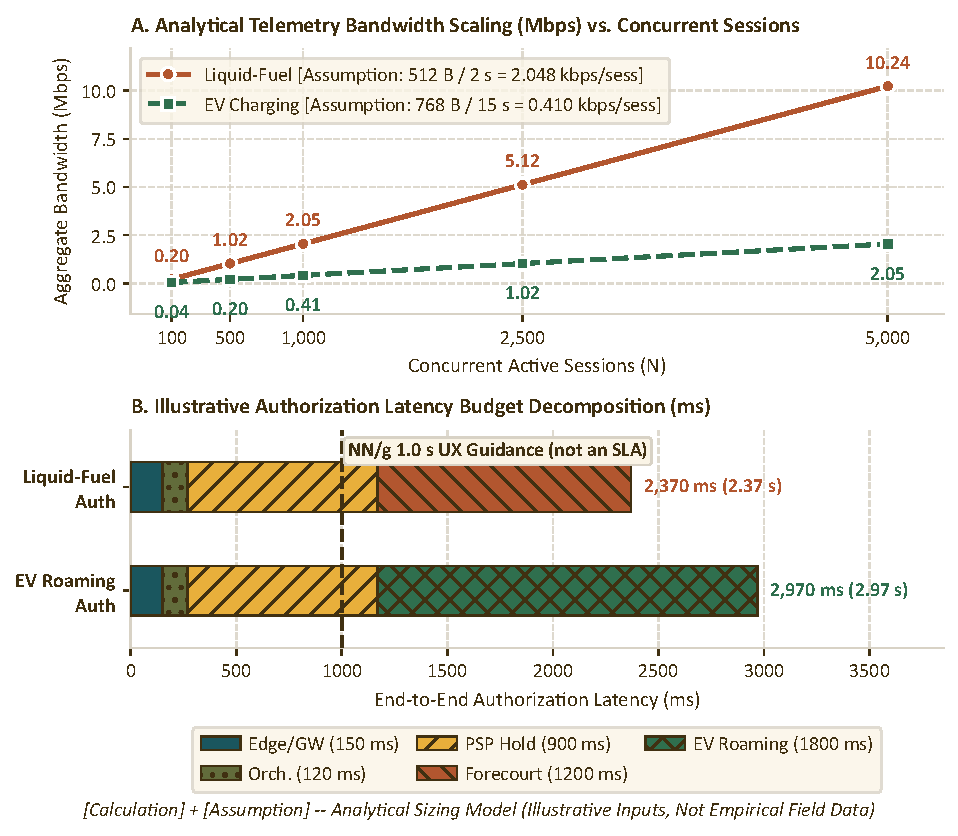
\includegraphics[width=0.88\linewidth]{figures/fig5_2_telemetry_sizing.pdf}
  \caption{Analytical Telemetry Bandwidth Scaling and Illustrative Authorization Latency Budget. \emph{Provenance}: \texttt{[Calculation]} derived from stated engineering \texttt{[Assumption]} inputs (not empirical field measurements); NN/g $1.0\;\text{s}$ UX guidance~\cite{nielsen1993responsetimes} shown for reference.}
  \label{fig:telemetry-sizing}
\end{figure}


\vspace{10pt}
% ==============================================================================
% Chapter 6: UX/UI Preliminary Flows, Visual Identity & Accessibility
% Indicative Space Budget: ~2.0 pages
% Status: Draft — Prepared by Research; Pending Partner Review
% ==============================================================================

\fgchapter{06}{Chapter 06 --- UX/UI \& Accessibility}{UX/UI Preliminary Flows, Visual Identity \& Accessibility}{Dual-energy mobile journeys, error-prevention guardrails, and WCAG 2.2 Level AA controls}{sec:ux-ui}

\subsection{Dual-Energy Mobile Journeys: Normal, Error, and Recovery States}
\label{sec:ux-journeys}

Outdoor forecourts and charging hubs impose high cognitive and environmental friction: bright sunlight, gloved or one-handed operation, time pressure, and the risk of costly misfueling. Fuel\&Go's conceptual mobile interface unifies ICE/Hybrid and EV journeys into a four-stage flow (\emph{Discover $\rightarrow$ Verify Bay $\rightarrow$ Monitor Live $\rightarrow$ Receipt}) while explicitly engineering error and recovery states (\texttt{FR-01}--\texttt{FR-06b}):

\begin{itemize}[leftmargin=1.4em, itemsep=2pt]
  \item \textbf{Normal Flow}: Drivers filter nearby stations by their saved \texttt{VehicleProfile} (\texttt{FR-01}, \texttt{FR-02}), scan a bay QR/NFC tag or confirm the bay number after a geofence check (\texttt{FR-03}), review an explicit pre-authorization summary, monitor live liters/kWh and running cost (\texttt{FR-04}), and receive an itemized digital receipt (\texttt{FR-05}).
  \item \textbf{Error Prevention (Slide~50 Guardrail)}: Incompatible fuel grades (e.g., diesel vs.\ gasoline) or mismatched EV connectors (e.g., CHAdeMO vs.\ CCS2) are disabled or hidden based on the active vehicle profile, requiring an explicit confirmation modal before authorization dispatch.
  \item \textbf{Fault \& Recovery States (\texttt{FR-06a}, \texttt{FR-06b})}: If PSP pre-authorization is explicitly declined or the operator explicitly rejects activation (\texttt{ABORTED\_VOID\_REQUESTED}), the UI prompts an alternative tokenized payment method and confirms the automated PSP hold-release request. Conversely, if an ambiguous authorization timeout or network drop occurs, the session enters \texttt{RECONCILING} (keeping the bay locked without blindly voiding the hold or retrying activation), displaying a persistent \emph{Reconciling Session} banner with a non-blocking status indicator (aligned with NN/g's $1.0\;\text{s}$--$10\;\text{s}$ feedback guidance~\cite{nielsen1993responsetimes}), disabled duplicate start controls, and a one-tap issue report linked to the session ID.
\end{itemize}

% ------------------------------------------------------------------------------
% FIGURE 6.1 HOOK FOR DESIGN AGENT (TikZ Vector Diagram #5 — Conceptual Mockup)
% 4-stage mobile journey + error/recovery callout states (Wrong Fuel Grade,
% Bay/Connector Mismatch, Timeout/Reconciling, Payment Decline).
% MUST be explicitly labeled "Conceptual Mockup".
% ------------------------------------------------------------------------------
\begin{figure}[!htbp]
  \centering
  % ==============================================================================
% figures/ux_journey_flow.tex
% TikZ Vector Diagram #5 (Figure 6.1): Compact Four-Stage Conceptual Mobile
% Screen-State Mockup + Error Prevention + Fault Recovery + WCAG 2.2 AA Strip
% Strictly <= 16.5cm wide; all labels >= 9.5pt; ZERO nested tikzpictures
% ==============================================================================
\begin{tikzpicture}[
  x=1cm, y=1cm,
  >=Stealth,
  phone/.style={
    rectangle, rounded corners=6pt,
    draw=#1, line width=1.15pt, fill=fgWhite,
    minimum width=3.65cm, minimum height=3.85cm,
    align=left, inner sep=0pt
  },
  guardbox/.style={
    rectangle, rounded corners=4pt,
    draw=#1, dashed, line width=1.1pt, fill=#1!8,
    minimum width=7.95cm, minimum height=1.82cm,
    align=left, inner sep=5pt,
    font=\fontsize{9.5pt}{10.8pt}\selectfont, text=fgEspresso
  },
  flowarrow/.style={draw=fgTeal, line width=1.2pt, ->}
]

% ------------------------------------------------------------------------------
% Top Conceptual Mockup Header Banner
% ------------------------------------------------------------------------------
\draw[fgAmber, line width=1.0pt, rounded corners=3pt, fill=fgCream]
  (0.0, 6.95) rectangle (16.30, 7.62);
\node[anchor=west, font=\fontsize{9.5pt}{10.8pt}\selectfont\bfseries, text=fgEspresso]
  at (0.22, 7.28) {Dual-Energy Mobile Screen-State Flow (ICE/Hybrid \& EV)};
\node[anchor=east, rectangle, rounded corners=2pt, fill=fgTeal, inner xsep=5pt, inner ysep=2pt,
      font=\fontsize{9.5pt}{10.5pt}\selectfont\bfseries, text=fgWhite]
  at (16.12, 7.28) {CONCEPTUAL MOCKUP};

% ------------------------------------------------------------------------------
% Row 1: Four-Stage Mobile Screen-State Mockup Cards
% ------------------------------------------------------------------------------
% Stage 1: Discover
\node[phone=fgTeal] (p1) at (1.85, 4.78) {};
\fill[fgTeal, rounded corners=4pt] (0.04, 6.16) rectangle (3.66, 6.68);
\node[font=\fontsize{9.5pt}{10.5pt}\selectfont\bfseries, text=fgWhite] at (1.85, 6.42) {1. Discover};
\node[anchor=north west, text width=3.35cm, font=\fontsize{9.5pt}{10.6pt}\selectfont, text=fgEspresso]
  at (0.14, 6.08) {%
  $\bullet$ Saved \texttt{VehicleProfile}\\
  $\bullet$ Map/list by fuel/plug\\
  $\bullet$ Live bay availability\\
  $\bullet$ Tariff preview (\texttt{FR-02})};

% Stage 2: Verify Bay
\node[phone=fgTerracotta] (p2) at (6.05, 4.78) {};
\fill[fgTerracotta, rounded corners=4pt] (4.24, 6.16) rectangle (7.86, 6.68);
\node[font=\fontsize{9.5pt}{10.5pt}\selectfont\bfseries, text=fgWhite] at (6.05, 6.42) {2. Verify Bay};
\node[anchor=north west, text width=3.35cm, font=\fontsize{9.5pt}{10.6pt}\selectfont, text=fgEspresso]
  at (4.34, 6.08) {%
  $\bullet$ QR / NFC bay scan\\
  $\bullet$ Geofence match\\
  $\bullet$ Pre-auth summary\\
  $\bullet$ \textbf{Slide 50} grade lock};

% Stage 3: Monitor Live
\node[phone=fgEcoGreen] (p3) at (10.25, 4.78) {};
\fill[fgEcoGreen, rounded corners=4pt] (8.44, 6.16) rectangle (12.06, 6.68);
\node[font=\fontsize{9.5pt}{10.5pt}\selectfont\bfseries, text=fgWhite] at (10.25, 6.42) {3. Monitor Live};
\node[anchor=north west, text width=3.35cm, font=\fontsize{9.5pt}{10.6pt}\selectfont, text=fgEspresso]
  at (8.54, 6.08) {%
  $\bullet$ Live L or kWh / kW\\
  $\bullet$ Running cost counter\\
  $\bullet$ EV SoC \& Remote Stop\\
  $\bullet$ Progress indicator};

% Stage 4: Digital Receipt
\node[phone=fgOlive] (p4) at (14.45, 4.78) {};
\fill[fgOlive, rounded corners=4pt] (12.64, 6.16) rectangle (16.26, 6.68);
\node[font=\fontsize{9.5pt}{10.5pt}\selectfont\bfseries, text=fgWhite] at (14.45, 6.42) {4. Digital Receipt};
\node[anchor=north west, text width=3.35cm, font=\fontsize{9.5pt}{10.6pt}\selectfont, text=fgEspresso]
  at (12.74, 6.08) {%
  $\bullet$ Metered total (\texttt{FR-05})\\
  $\bullet$ Exact PSP capture\\
  $\bullet$ Hold-release notice\\
  $\bullet$ 1-tap issue report};

% Connecting Arrows
\draw[flowarrow] (p1.east) -- (p2.west);
\draw[flowarrow] (p2.east) -- (p3.west);
\draw[flowarrow] (p3.east) -- (p4.west);

% ------------------------------------------------------------------------------
% Row 2: Error Prevention (Slide 50) & Fault Recovery (FR-06a/b)
% ------------------------------------------------------------------------------
\node[guardbox=fgTerracotta, text width=7.60cm] (err) at (4.00, 1.62) {%
  \textbf{\textcolor{fgTerracotta}{Error Prevention (Slide 50 Guardrail)}}\\
  Incompatible fuel grades (e.g., Diesel vs.\ Gasoline) or EV connectors (CHAdeMO vs.\ CCS2) are disabled/hidden per active vehicle profile; explicit confirmation modal required before dispatch.};

\node[guardbox=fgTextAmber, text width=7.60cm] (rec) at (12.30, 1.62) {%
  \textbf{\textcolor{fgTextAmber}{Fault Recovery (\texttt{FR-06a} / \texttt{FR-06b})}}\\
  Persistent \emph{Timeout / Reconciling} banner + disabled duplicate start tap + automated PSP hold-release notice + session-linked 1-tap issue report.};

% Subtle links from Verify/Monitor to Guardrails
\draw[fgTerracotta, dashed, line width=0.9pt, ->] (p2.south) -- (6.05, 2.55);
\draw[fgTextAmber, dashed, line width=0.9pt, ->] (p3.south) -- (10.25, 2.55);

% ------------------------------------------------------------------------------
% Row 3: WCAG 2.2 Level AA Accessibility Strip
% ------------------------------------------------------------------------------
\draw[fgTeal, line width=1.0pt, rounded corners=3pt, fill=fgTealTint!70]
  (0.0, -0.48) rectangle (16.30, 0.42);
\node[anchor=center, align=center, text width=15.6cm, font=\fontsize{9.5pt}{10.8pt}\selectfont, text=fgEspresso]
  at (8.15, -0.03) {%
  \textbf{\textcolor{fgTeal}{WCAG 2.2 Level AA Accessibility Strip:}} $\ge 4.5{:}1$ Normal Text Contrast (SC 1.4.3)\\
  $\ge 24\times 24$ CSS px Pointer Targets (SC 2.5.8) $\;\cdot\;$ Non-Color Icons \& $\ge 3{:}1$ UI Contrast (SC 1.4.11)};

\end{tikzpicture}

  \caption{Dual-Energy Mobile User Journey, Error-Prevention Guardrails, and Fault-Recovery States (\emph{Conceptual Mockup --- Not an Implemented UI}).}
  \label{fig:ux-journey}
\end{figure}

\subsection{Visual Identity Alignment and WCAG 2.2 Level AA Accessibility}
\label{sec:ux-accessibility}

Fuel\&Go's conceptual UI adapts the warm earthy palette of the original product presentation (\texttt{Fuel\&Go Whole Tasks.pptx}) while hardening contrast for outdoor legibility and accessibility-challenged drivers (Presentation Slide~4). All accessibility controls are anchored directly to W3C \textbf{WCAG~2.2 Level~AA}~\cite{w3c2023wcag22} (verified directly against the W3C Recommendation):

\begin{itemize}[leftmargin=1.4em, itemsep=2pt]
  \item \textbf{Text Contrast (SC~1.4.3)}: Normal text requires $\ge 4.5{:}1$ contrast and large text requires $\ge 3{:}1$~\cite{w3c2023wcag22}. Deterministic relative-luminance calculations confirm that Deep Espresso (\texttt{\#403011}) on White (\texttt{\#FFFFFF}, $12.74{:}1$) and Cream (\texttt{\#F6EBD4}, $10.77{:}1$) exceeds AAA, while White on Olive (\texttt{\#626C3B}, $5.63{:}1$) and Darkened Amber (\texttt{\#8C5A00}) on White ($5.87{:}1$) pass AA. Low-contrast golden amber (\texttt{\#E8AF3B}, $1.67{:}1$ on cream) is restricted strictly to non-text borders and graphical accents.
  \item \textbf{Non-Text Contrast (SC~1.4.11) \& Color Independence}: UI borders, focus rings, and status icons maintain $\ge 3{:}1$ contrast~\cite{w3c2023wcag22}, and every fuel/EV status indicator pairs color with distinct iconography and text labels so colorblind drivers never rely on hue alone.
  \item \textbf{Pointer Target Size (SC~2.5.8)}: Interactive controls (bay selectors, stop-charging button, fault-recovery actions) enforce at least $24 \times 24\;\text{CSS~px}$ minimum pointer target size~\cite{w3c2023wcag22}, with generous spacing for reliable outdoor one-handed touch input.
\end{itemize}

Table~\ref{tab:ux-accessibility} maps driver error-prevention guardrails and WCAG~2.2 Level~AA criteria to planned verification methods.

\begin{table}[htbp]
  \centering
  \caption{Driver Error-Prevention Guardrails and WCAG 2.2 Level AA Accessibility Matrix.}
  \label{tab:ux-accessibility}
  \small
  \begin{tabularx}{\linewidth}{@{}P{28mm} P{26mm} L P{28mm}@{}}
    \toprule
    \rowcolor{fgOlive}
    \fgtableheader{UX / Accessibility Area} & \fgtableheader{Governing Basis} & \fgtableheader{Proposed Interface Control} & \fgtableheader{Planned Verification} \\
    \midrule
    \textbf{Misfueling \& Connector Guardrail} & Slide~50; \texttt{FR-01}, \texttt{FR-03} & Hide/disable incompatible fuel grades or EV plugs; require explicit bay + energy-type confirmation before start. & Wireframe task-flow walkthrough \& heuristic audit. \\
    \textbf{Timeout \& Payment Fault Recovery} & \texttt{FR-06a}, \texttt{FR-06b}; NN/g~\cite{nielsen1993responsetimes} & Disable duplicate start taps; display non-blocking progress/reconciliation banner; expose session-linked issue form. & State-machine UI walkthrough \& fault-injection test. \\
    \textbf{Text \& Outdoor Legibility} & WCAG~2.2 SC~1.4.3~\cite{w3c2023wcag22}; \texttt{NFR-07a} & Enforce $\ge 4.5{:}1$ normal text contrast (\texttt{\#403011} on white/cream; \texttt{\#8C5A00} links); ban \texttt{\#E8AF3B} for text. & Deterministic luminance check \& visual inspection. \\
    \textbf{Non-Text UI \& Colorblind Safety} & WCAG~2.2 SC~1.4.11~\cite{w3c2023wcag22} & Maintain $\ge 3{:}1$ contrast on controls/icons; pair every status color with explicit text and distinct shape/icon. & Grayscale render audit \& contrast calculation. \\
    \textbf{Touch Target Ergonomics} & WCAG~2.2 SC~2.5.8~\cite{w3c2023wcag22}; Slide~4 & Enforce $\ge 24 \times 24\;\text{CSS~px}$ minimum pointer target size with clear spacing for one-handed forecourt use. & Component spec audit \& future usability testing. \\
    \bottomrule
  \end{tabularx}
\end{table}


\vspace{10pt}
% ==============================================================================
% sections/sec07_security_safety.tex
% Chapter 7 — Security, Physical Safety, Privacy & Regulatory Compliance (~2.0 pp)
% ==============================================================================
\fgchapter{07}{Cyber-Physical Risk Posture}{Security, Physical Safety, Privacy \& Regulatory Compliance}{Trust boundaries, STRIDE threat controls, payment-scope limits, hardware safety isolation, and jurisdiction-dependent privacy}{sec:security-safety}

Operating a unified mobile platform that authorizes physical liquid-fuel dispensing and high-voltage EV charging introduces cyber-physical, financial, and privacy risks that extend beyond conventional consumer apps. Because Fuel\&Go is a \emph{Conceptual System Design}, all security controls, safety assumptions, and compliance architectures below represent proposed engineering baselines requiring independent penetration testing, hardware-in-the-loop (HIL) validation, and formal legal review before pilot deployment.

\subsection{Trust Boundaries, Payment Tokenization Scope \& Hardware Safety Isolation}
Figure~\ref{fig:safety-trust-boundary} partitions Fuel\&Go into four explicit trust zones: (Z1)~the untrusted driver mobile device and physical bay environment; (Z2)~the Fuel\&Go cloud orchestration platform; (Z3)~the external Payment Service Provider (PSP) vault; and (Z4)~the station operator's local forecourt/EVSE hardware safety domain.

\begin{figure}[htbp]
  \centering
  % ==============================================================================
% figures/safety_trust_boundary.tex
% Figure 7.1 — Trust Boundaries, PSP Tokenization Scope & Autonomous Local
%              Hardware Safety Interlock Isolation (NFR-06)
% Constraints: ZERO nested tikzpicture, <= 16.5cm width, >= 9.5pt labels,
%              Fuel&Go palette, grayscale-safe (distinct border styles & fills)
% ==============================================================================
\begin{tikzpicture}[
  x=1cm, y=1cm,
  font=\sffamily,
  >=Stealth,
  zonebox/.style={
    rounded corners=3pt,
    line width=1.0pt,
    align=center
  },
  comp/.style={
    rectangle,
    rounded corners=2.5pt,
    draw=fgEspresso,
    fill=fgWhite,
    line width=0.7pt,
    align=center,
    font=\sffamily\fontsize{9.5pt}{11pt}\selectfont,
    inner sep=4pt
  },
  lbl/.style={
    font=\sffamily\bfseries\fontsize{9.5pt}{11pt}\selectfont,
    align=center
  },
  edge/.style={
    ->,
    line width=0.95pt,
    draw=fgEspresso
  },
  edgeBi/.style={
    <->,
    line width=0.95pt,
    draw=fgEspresso
  },
  note/.style={
    font=\sffamily\fontsize{9.5pt}{10.8pt}\selectfont,
    align=center,
    fill=fgWhite,
    inner sep=1.5pt
  }
]

% --- ZONE 1: Untrusted Client & Edge (Left) ---
\draw[zonebox, fill=fgSoftCream, draw=fgAmber, dashed]
  (0.0, 0.2) rectangle (4.3, 6.9);
\node[lbl, text=fgTextAmber] at (2.15, 6.55) {Z1: Untrusted Client};

\node[comp, text width=3.5cm, draw=fgTeal, fill=fgTealTint] (mob) at (2.15, 5.15)
  {\textbf{Fuel\&Go Mobile App}\\OWASP MASVS v2.1.0\\TLS 1.3 + Cert Pinning};

\node[comp, text width=3.5cm, draw=fgOlive, fill=fgPaleSage] (sdk) at (2.15, 3.05)
  {\textbf{PSP Client SDK}\\Direct PAN Capture\\(No PAN to Backend)};

\node[comp, text width=3.5cm, draw=fgEspresso, fill=fgWhite] (bay) at (2.15, 1.15)
  {\textbf{Bay Verification}\\QR/NFC + Geofence\\+ Manual Bay ID};

% --- ZONE 2: Fuel&Go Cloud Platform (Center-Left) ---
\draw[zonebox, fill=fgTealTint!55, draw=fgTeal, solid]
  (4.9, 2.3) rectangle (10.5, 6.9);
\node[lbl, text=fgTeal] at (7.7, 6.55) {Z2: Fuel\&Go Cloud (Non-CDE)};

\node[comp, text width=4.8cm, draw=fgTeal, fill=fgWhite] (gw) at (7.7, 5.45)
  {\textbf{API Gateway \& Auth}\\OWASP API Top 10 (BOLA, Rate Limit)};

\node[comp, text width=4.8cm, draw=fgTeal, fill=fgWhite] (orch) at (7.7, 3.55)
  {\textbf{Session Orchestrator \& Ledger}\\Idempotency Keys, Hold/Capture\\Reconciliation (Tokens Only)};

% --- ZONE 3: PCI DSS CDE / PSP Vault (Bottom-Center) ---
\draw[zonebox, fill=fgPaleSage, draw=fgOlive, densely dotted, line width=1.2pt]
  (4.9, 0.2) rectangle (10.5, 2.05);
\node[comp, text width=4.8cm, draw=fgOliveDark, fill=fgWhite] (psp) at (7.7, 1.38)
  {\textbf{Tokenized PSP APIs} (PCI DSS v4.0.1)\\PAN Vault, Pre-Auth Hold, Capture};
\node[lbl, text=fgOliveDark] at (7.7, 0.45) {Z3: External PSP Vault (PCI DSS CDE)};

% --- ZONE 4: Autonomous Local Hardware Safety Domain (Right) ---
\draw[zonebox, fill=fgTerraTint, draw=fgTerracotta, line width=1.4pt]
  (11.2, 0.2) rectangle (16.4, 6.9);
\node[lbl, text=fgTerracotta] at (13.8, 6.55) {Z4: Local Safety Domain};

\node[comp, text width=4.5cm, draw=fgTerracotta, fill=fgWhite] (fcc) at (13.8, 5.25)
  {\textbf{Forecourt / EV CPMS}\\IFSF Gateway / OCPI Backend\\(Remote Start/Stop Only)};

\draw[draw=fgTerracotta, line width=1.1pt, dash dot]
  (11.45, 4.18) -- (16.15, 4.18);
\node[note, fill=fgTerraTint, text=fgTerracotta, font=\sffamily\bfseries\fontsize{9.5pt}{10.5pt}\selectfont]
  at (14.25, 4.18) {NFR-06 Hardware Isolation};

\node[comp, text width=4.5cm, draw=fgTerracotta, fill=fgWhite] (hwfuel) at (13.8, 2.72)
  {\textbf{Fuel Dispenser Interlocks}\\Hardware E-Stop, Overfill\\\& Vapor-Recovery Cutoff};

\node[comp, text width=4.5cm, draw=fgEcoGreen, fill=fgEcoTint] (hwev) at (13.8, 1.02)
  {\textbf{EVSE Safety Interlocks}\\Ground-Fault (RCD), HV\\Contactor \& Thermal Cutoff};

% --- ARROWS & TRUST BOUNDARY CROSSINGS ---
\draw[edgeBi, fgTeal] (mob.east) -- (gw.west);
\draw[edge, fgOliveDark, dashed] (sdk.east) -- (4.6, 3.05) |- (psp.west);
\draw[edgeBi, fgTeal] (gw.south) -- (orch.north);
\draw[edgeBi, fgOliveDark] (orch.south) -- (psp.north);
\draw[edgeBi, fgTerracotta] (orch.east) -- ++(0.35,0) |- (fcc.west);
\draw[edge, fgEspresso, dotted, line width=0.8pt] (bay.north) -- (sdk.south);

% Autonomous indicator (no cloud dependency; shifted left to avoid label collision)
\draw[edge, fgTerracotta, line width=0.9pt] ([xshift=-1.65cm]fcc.south) -- ([xshift=-1.65cm]hwfuel.north);
\node[note, fill=fgTerraTint, text=fgEspresso] at (14.25, 3.68) {No Safety Override};

\end{tikzpicture}

  \caption{Fuel\&Go Trust Boundaries, PSP Tokenization Scope (\texttt{PCI~DSS~v4.0.1}~\cite{pcissc2024pcidss401}), Mobile/API Security (\texttt{OWASP MASVS~v2.1.0}~\cite{owasp2024masvs}, \texttt{OWASP API Top~10~2023}~\cite{owasp2023apitop10}), and Autonomous Local Hardware Safety Interlock Isolation (\texttt{NFR-06}). \emph{[Proposed Architecture]}}
  \label{fig:safety-trust-boundary}
\end{figure}

\textbf{Payment Card Scope Reduction Limits (PCI DSS v4.0.1):} Under PCI~DSS~v4.0.1~\cite{pcissc2024pcidss401}, Fuel\&Go delegates raw Primary Account Number (PAN) capture and storage to a certified PSP client SDK and external vault (Z3), returning only non-sensitive surrogate tokens to the Fuel\&Go backend (Z2). While tokenization concentrates cardholder data at the PSP and narrows the Cardholder Data Environment (CDE), \emph{tokenization alone does not establish PCI~DSS compliance}. Compliant mobile SDK integration, TLS transport protection, operational access controls, vulnerability management, and formal merchant self-assessment or QSA audit remain mandatory.

\textbf{Mobile \& API Security Baselines:} Mobile clients target OWASP~MASVS~v2.1.0~\cite{owasp2024masvs} controls (secure keystore credential storage, TLS~1.3 certificate pinning, tamper/root detection, and \texttt{MASVS-PRIVACY} data minimization). Backend endpoints enforce OWASP~API Security Top~10 (2023)~\cite{owasp2023apitop10} defenses, prioritizing object-level authorization checks against Broken Object Level Authorization (API1: BOLA), short-lived OAuth~2.0/OIDC tokens (API2), rate limiting (API4), and strict schema validation when consuming third-party operator APIs (API10).

\textbf{Autonomous Local Hardware Safety Isolation (\texttt{NFR-06}):} Fuel\&Go \emph{never} assumes responsibility for physical safety interlocks. Certified local forecourt emergency-stop (E-stop) switches, nozzle overfill and vapor-recovery shutoffs, and EVSE ground-fault (RCD), thermal, and high-voltage contactor cutoffs operate autonomously within Z4. A cloud outage, mobile battery failure, or network partition cannot disable local safety cutoffs or force uncontrolled energy delivery.

\subsection{Condensed STRIDE Threat Model \& Residual Risk Posture}
Table~\ref{tab:stride-threats} summarizes six priority threats across the STRIDE taxonomy, mapping proposed controls, residual risks, key design assumptions, and required future validation.

\begin{table}[htbp]
  \centering
  \caption{Condensed STRIDE Threat Model, Proposed Controls, Residual Risks, Assumptions \& Required Validation. \emph{[Conceptual Design]}}
  \label{tab:stride-threats}
  {\footnotesize
  \begin{tabularx}{\linewidth}{@{}P{24mm} P{36mm} P{32mm} P{30mm} L@{}}
    \toprule
    \rowcolor{fgOlive}
    \fgtableheader{Threat (STRIDE)} & \fgtableheader{Proposed Controls} & \fgtableheader{Residual Risks} & \fgtableheader{Key Assumptions} & \fgtableheader{Required Future Validation} \\
    \midrule
    \textbf{QR Sticker Replacement} (Spoofing) & Signed station/bay payloads; geofence proximity check; in-app bay-number confirmation; operator bay-status cross-check. & Social-engineered driver ignores bay mismatch or approves wrong pump in adjacent lane. & Operator API exposes real-time bay ID and station coordinates. & Field usability testing and red-team physical spoofing drills at pilot stations. \\
    \rowcolor{fgSoftCream}
    \textbf{GPS Spoofing} (Spoofing / Tampering) & Server-side plausibility checks (velocity/jump); combine GPS with QR/NFC scan; OS integrity attestation (MASVS~\cite{owasp2024masvs}). & Rooted/jailbroken devices may bypass client attestation and trigger remote bay unlock. & Local bay presence is reinforced by physical nozzle lift or EV cable plug-in. & Mobile penetration testing against mock-location and instrumentation frameworks. \\
    \textbf{Session Hijacking / BOLA} (Info Disc. / EoP) & Short-lived bearer tokens; strict per-object ownership checks (OWASP API1~\cite{owasp2023apitop10}); device-bound refresh tokens. & Compromised unlocked phone allows unauthorized session start within active token window. & Biometric or OS PIN re-authentication protects payment/session confirmation. & Automated API authorization fuzzing and independent OWASP API Top~10 pentest. \\
    \rowcolor{fgSoftCream}
    \textbf{Replay / Duplicate Settlement} (Tampering / Repud.) & Client-generated idempotency keys reused on retries; durable ledger deduplication; PSP webhook signature verification. & Downstream operator/FCC lacking native idempotency may double-authorize if timeout occurs. & Authoritative operator/CDR reconciliation resolves ambiguous timeouts before capture. & Fault-injection testing (network drop, duplicate webhook, timeout) in sandbox/HIL. \\
    \textbf{API Abuse / Resource Exhaustion} (DoS) & API gateway rate limiting (OWASP API4~\cite{owasp2023apitop10}); per-user concurrent session caps; circuit breakers on operator adapters. & Coordinated botnet could degrade discovery APIs or exhaust operator rate quotas. & Cloud WAF and autoscaling absorb volumetric traffic spikes. & Load and stress testing against rate-limit and circuit-breaker thresholds. \\
    \rowcolor{fgSoftCream}
    \textbf{Unsafe Operator API Consumption} (Tampering) & Strict JSON schema validation; mTLS/signed webhooks (OWASP API10~\cite{owasp2023apitop10}); anomaly bounds on meter values. & Compromised partner CPMS/FCC could inject falsified meter totals or malicious payloads. & Partner operators maintain isolated, patched CPMS/FCC infrastructure. & Contract testing with malformed/adversarial partner payloads in staging. \\
    \bottomrule
  \end{tabularx}
  }
\end{table}

\subsection{Jurisdiction-Dependent Privacy \& Regulatory Compliance}
Privacy and data-protection obligations depend strictly on the confirmed deployment jurisdiction rather than assuming a single global regime:
\begin{itemize}[leftmargin=12pt, itemsep=2pt, topsep=2pt]
  \item \textbf{Israel Protection of Privacy Law, 5741--1981 (Amendment~13)~\cite{israel1981ppl}:} Under the working territorial launch assumption in Israel (pending formal partner confirmation), Fuel\&Go falls under Israeli statutory privacy governance enforced by the Privacy Protection Authority (PPA). Amendment~13 (enacted 2024, effective 2025) introduces direct administrative monetary sanctions and mandatory Data Protection Officer (DPO) obligations for qualifying databases, requiring strict data minimization for location trails, vehicle profiles, and transaction logs.
  \item \textbf{EU General Data Protection Regulation (GDPR)~\cite{eu2016gdpr} (Conditional):} GDPR applies extraterritorially under Article~3 \emph{only} if Fuel\&Go establishes an EU entity, offers services to data subjects in the EU, or monitors their behavior within the EU. It does \emph{not} apply automatically to an Israel-only deployment, though adopting privacy-by-design (purpose limitation, retention caps, and user export/deletion controls) lowers future EU expansion friction.
\end{itemize}


\vspace{10pt}
% ==============================================================================
% sections/sec08_verification_qa.tex
% Chapter 8 — Planned Product Verification vs. Actual Report QA (~2.0 pp)
% ==============================================================================
\fgchapter{08}{Dual-Track Verification}{Planned Product Verification vs. Actual Report QA \& Red-Team Summary}{Strict separation of conceptual product test plans from executed Assignment 02 document verification}{sec:verification-qa}

A core engineering governance principle of this report is maintaining a strict boundary between \textbf{Track~1 (Planned Product Verification)}, which defines conceptual, unexecuted tests for the future Fuel\&Go software and station integrations, and \textbf{Track~2 (Actual Report QA \& Red-Team)}, which records verified quality-assurance audits executed on this Assignment~02 LaTeX deliverable. A clean PDF build never validates runtime product behavior, safety interlocks, or payment settlement accuracy.

\subsection{Track 1: Planned Product Verification (Conceptual / Unexecuted)}
Table~\ref{tab:traceability-matrix} maps core functional requirements (\texttt{FR-01}--\texttt{FR-06b}) and non-functional requirements (\texttt{NFR-01a}--\texttt{NFR-07b}) to conceptual architecture components, proposed future test levels, and acceptance criteria in alignment with ISO/IEC/IEEE 29148:2018~\cite{iso29148_2018} traceability practices. \emph{Status: All product tests below are unexecuted design plans.}

\begin{table}[htbp]
  \centering
  \caption{Requirements-to-Architecture-to-Planned-Verification Traceability Matrix (\emph{Track~1: Conceptual / Unexecuted Product Verification}).}
  \label{tab:traceability-matrix}
  {\footnotesize
  \begin{tabularx}{\linewidth}{@{}P{20mm} P{36mm} P{32mm} L@{}}
    \toprule
    \rowcolor{fgTeal}
    \fgtableheader{Req. ID} & \fgtableheader{Architecture Component} & \fgtableheader{Proposed Test Level} & \fgtableheader{Conceptual Acceptance Criteria (Unexecuted)} \\
    \midrule
    \texttt{FR-01} & Mobile Client, Auth Service, Vehicle Profile DB & Unit, Integration, Security Test & User registers/authenticates; vehicle energy type (ICE/PHEV/BEV) and compatible fuel/connector constraints persist accurately. \\
    \rowcolor{fgSoftCream}
    \texttt{FR-02} & Discovery Service, PostGIS~\cite{postgis2025docs}, OCPI/FCC Adapters & Integration, Geospatial Load Test & Map/list returns stations filtered by fuel grade or EV connector type with live availability status from mock operator feeds. \\
    \texttt{FR-03} & Session Orchestrator, Bay Verifier, Adapter Layer & Integration, Fault-Injection, HIL & Valid QR/bay match triggers pre-auth hold and remote unlock; mismatched fuel/connector or timeout enters safe reconciliation. \\
    \rowcolor{fgSoftCream}
    \texttt{FR-04} & Telemetry Streamer (WebSocket~\cite{rfc6455}), Redis~\cite{redis2025docs} & Integration, Endurance, Simulator & Live liters/cost (ICE) or kWh/kW/SoC (EV) updates stream smoothly; disconnect triggers automatic reconnect and state resync. \\
    \texttt{FR-05} & Payment Service, Ledger DB, PSP Adapter & Sandbox Payment, Chaos Test & Idempotent capture settles exact delivered amount; unused pre-auth hold releases promptly; digital receipt matches ledger. \\
    \rowcolor{fgSoftCream}
    \texttt{FR-06a/b} & Orchestrator, Support/Dispute Module, RabbitMQ~\cite{rabbitmq2025docs} & Fault-Injection, E2E Workflow & Network drops, charger faults, or ambiguous timeouts trigger deterministic reconciliation and structured user dispute logging. \\
    \texttt{NFR-01a/b} & API Gateway, Orchestrator, Operator Adapters & Load \& Latency Benchmark & Measured P95 discovery and authorization latencies evaluated against provisional UX responsiveness thresholds~\cite{nielsen1993responsetimes}. \\
    \rowcolor{fgSoftCream}
    \texttt{NFR-02/03} & Cloud Cluster, Multi-AZ DB, Circuit Breakers & Chaos / Failover Test & Service availability and horizontal scaling verified under simulated regional failover and concurrent session bursts. \\
    \texttt{NFR-04/05} & Mobile SDK, API Gateway, PSP Vault & OWASP MASVS/API Pentest, PCI Audit & Zero PAN exposure in Fuel\&Go logs/DB~\cite{pcissc2024pcidss401}; zero critical BOLA or auth bypasses~\cite{owasp2024masvs,owasp2023apitop10}. \\
    \rowcolor{fgSoftCream}
    \texttt{NFR-06} & Local Forecourt Dispenser \& EVSE Hardware & Certified Station HIL Safety Test & Physical E-stop, overfill/vapor cutoff, and EVSE ground-fault trips halt energy delivery during simulated cloud/mobile outage. \\
    \texttt{NFR-07a/b} & Mobile UI (Flutter~\cite{flutter2025docs}), Design System & Accessibility Audit (WCAG~2.2~\cite{w3c2023wcag22}) & Text contrast $\ge 4.5{:}1$, non-text $\ge 3{:}1$, touch targets $\ge 24\times 24$~CSS~px, and screen-reader traversal pass AA checks. \\
    \bottomrule
  \end{tabularx}
  }
\end{table}

\subsection{Track 2: Actual Report QA \& Red-Team Summary (Executed)}
To ensure academic integrity, deterministic typesetting, and zero fabrication on this Assignment~02 report, an independent read-only \texttt{detector} agent audited deliverables across Phases~0--5, logging defects in \texttt{qa/defects.json} and \texttt{qa/DEFECTS.md}, while \texttt{fixer} remediated root causes and documented mandatory 5-part incident records (\texttt{qa/incidents/INC-DEF-001.md}--\texttt{INC-DEF-010.md}). Per the outline's anti-padding rule, no decorative QA chart is included; Table~\ref{tab:actual-qa-summary} reports the exact recorded audit outcomes.

\begin{table}[htbp]
  \centering
  \caption{Actual Report QA \& Incident Remediation Summary (\emph{Track~2: Executed Document Audits, Phases~0--5}).}
  \label{tab:actual-qa-summary}
  {\footnotesize
  \begin{tabularx}{\linewidth}{@{}P{24mm} P{26mm} P{22mm} L@{}}
    \toprule
    \rowcolor{fgOlive}
    \fgtableheader{Audit Phase / Artifact} & \fgtableheader{QA Families Checked} & \fgtableheader{Defects Logged / Closed} & \fgtableheader{Verified Root-Cause Remediations \& Current Status} \\
    \midrule
    \textbf{Phase 3 Research} (\texttt{references.bib}, \texttt{RESEARCH\_NOTES.md}) & \texttt{qa-citations}, Zero-Fabrication & \texttt{DEF-001}--\texttt{DEF-004} (4 / 4 Closed) & Removed dangling unverified Israel key; split OCPI facts from assumptions; documented IEA charger density; standardized \texttt{biblatex-ieee} entry types. \\
    \rowcolor{fgSoftCream}
    \textbf{Phase 5 Visual Preview} (\texttt{visual\_\-preview.pdf}) & \texttt{qa-typeset}, \texttt{qa-img}, \texttt{qa-cls-version} & \texttt{DEF-005} (1 / 1 Closed) & Eliminated $13.19\text{pt}$ overfull \texttt{\textbackslash hbox} in TikZ architecture preview while preserving $\ge 8.5\text{pt}$ labels and grayscale legibility. \\
    \textbf{Chapters 1--3 Draft} (\texttt{draft\_ch1\_3.pdf} v1/v2) & \texttt{qa-img}, \texttt{qa-citations}, \texttt{qa-table}, \texttt{qa-typeset} & \texttt{DEF-006}--\texttt{DEF-010} (5 / 5 Closed) & Fixed missing \texttt{FR-06} link and nested-TikZ icon distortion (\texttt{DEF-006/009}); purged unverified Israel percentages and tagged Fig.~2.1 calculation (\texttt{DEF-007}); fixed narrow-column justification (\texttt{DEF-008}); added \texttt{placeins} float barrier to \texttt{nextmind-pdr.cls} v0.3.2 (\texttt{DEF-010}). \\
    \rowcolor{fgSoftCream}
    \textbf{Phase 6 Full Report} (\texttt{main.pdf}, 25 pp.) & Full 8 QA Families + Red-Team & \texttt{DEF-011}--\texttt{DEF-015} (5 Logged, Remediated) & Detector audited all 25 pages: factual, citation, math, and build checks passed; 5 visual/ToC layout defects (\texttt{DEF-011}--\texttt{DEF-015}) remediated by Fixer (\texttt{INC-DEF-011}--\texttt{015}), awaiting final Detector retest. \\
    \bottomrule
  \end{tabularx}
  }
\end{table}

\begin{sagebox}[Epistemic \& Governance Boundary]
  Ten defects (\texttt{DEF-001}--\texttt{DEF-010}) were independently closed across Phases~0--5. Five Phase~6 layout/diagram defects (\texttt{DEF-011}--\texttt{DEF-015}) were logged by Detector on \texttt{main.pdf} and remediated by Fixer; final closure remains pending independent Detector retest.
\end{sagebox}


\vspace{10pt}
% ==============================================================================
% sections/sec09_plan_conclusions.tex
% Chapter 9 — Product Delivery Plan, Risk Register, Roadmap & Conclusions (~1.5 pp)
% ==============================================================================
\fgchapterflow{09}{Execution Strategy}{Product Delivery Plan, Risk Register, Roadmap \& Conclusions}{Prioritized product risks, phased delivery milestones, extension boundaries, and go/no-go readiness criteria}{sec:plan-conclusions}

This chapter outlines the conceptual \textbf{Fuel\&Go Product Delivery Plan}—explicitly distinct from the academic production of this Assignment~02 report—alongside a prioritized risk register, a phased product roadmap, and executive go/no-go conclusions.

\subsection{Prioritized Product \& Integration Risk Register}
Following standard engineering risk-scoring practice, each risk in Table~\ref{tab:risk-register} is evaluated via $R = P \times I$ on a 1--5 scale for Probability ($P$) and Impact ($I$). \emph{All $P$, $I$, and $R$ values are explicitly tagged \texttt{[Assumption]} as subjective engineering judgments rather than empirical actuarial rates.}

\begin{table}[htbp]
  \centering
  \caption{Prioritized Fuel\&Go Product \& Integration Risk Register ($R = P \times I$, 1--5 Scale, \emph{[Assumption]}).}
  \label{tab:risk-register}
  {\footnotesize
  \begin{tabularx}{\linewidth}{@{}P{11mm} P{34mm} P{16mm} P{48mm} L@{}}
    \toprule
    \rowcolor{fgOlive}
    \fgtableheader{ID} & \fgtableheader{Risk Description} & \fgtableheader{$P \times I = R$} & \fgtableheader{Proposed Mitigation Strategy} & \fgtableheader{Residual Exposure} \\
    \midrule
    \texttt{RSK-01} & \textbf{Partner Onboarding Delay:} Fuel chains or EV CPOs decline or delay API/sandbox access. & $4 \times 5 = 20$ & Target one anchor fuel partner and one OCPI-compliant EV CPO for Phase~2 pilot; decouple via adapter pattern. & High commercial dependency; may delay pilot launch. \\
    \rowcolor{fgSoftCream}
    \texttt{RSK-02} & \textbf{Proprietary Forecourt Variance:} Legacy FCC/POS gateways deviate from IFSF~\cite{ifsf_specs}. & $4 \times 4 = 16$ & Isolate vendor-specific dialects inside per-operator forecourt adapters; validate in vendor HIL lab. & Adapter maintenance overhead per fuel chain. \\
    \texttt{RSK-03} & \textbf{Ambiguous Timeout / Orphaned Holds:} Network drop during remote unlock causes double-charge or stuck hold. & $3 \times 5 = 15$ & Enforce reusable idempotency keys, durable reconciliation state, and automated hold-release jobs. & Temporary driver frustration during manual dispute resolution. \\
    \rowcolor{fgSoftCream}
    \texttt{RSK-04} & \textbf{Physical QR Tampering:} Attacker overlays fraudulent QR sticker on unattended bay. & $3 \times 4 = 12$ & Require geofence match, signed QR payloads, and explicit bay-number confirmation in UI. & Social-engineering risk if driver ignores bay mismatch. \\
    \texttt{RSK-05} & \textbf{Privacy / PCI Scope Drift:} Accidental logging of PANs or excessive location retention~\cite{pcissc2024pcidss401,israel1981ppl}. & $2 \times 5 = 10$ & Strict PSP SDK tokenization, automated log scrubbing, data-retention TTLs, and pre-pilot compliance audit. & Ongoing audit and DPO governance cost. \\
    \bottomrule
  \end{tabularx}
  }
\end{table}

\subsection{Phased Fuel\&Go Product Delivery Roadmap}
Table~\ref{tab:product-roadmap} sequences Fuel\&Go from Core MVP to commercial rollout and source-supported extensions. All phase durations are preliminary planning estimates (\texttt{[Assumption]}). Unsupported or unapproved features—\texttt{EXT-01} (convenience-store food/coffee pre-ordering), consolidated corporate VAT invoicing, a standalone station-operator web dashboard, and the AI Guidance Assistant—remain \emph{excluded/quarantined} outside this roadmap unless formally approved in future scope governance.

\begin{table}[htbp]
  \centering
  \caption{Phased Fuel\&Go Product Delivery Roadmap (\emph{Conceptual Product Plan; Durations [Assumption]}).}
  \label{tab:product-roadmap}
  {\footnotesize
  \begin{tabularx}{\linewidth}{@{}P{24mm} P{22mm} P{54mm} L@{}}
    \toprule
    \rowcolor{fgTeal}
    \fgtableheader{Delivery Phase} & \fgtableheader{Est. Window} & \fgtableheader{Core Deliverables \& Scope} & \fgtableheader{Phase Exit / Readiness Gate} \\
    \midrule
    \textbf{Phase 1: Core MVP Build} & Months 1--4 \emph{[Assumption]} & Mobile app (\texttt{FR-01}--\texttt{FR-06b}), session orchestrator, PostGIS discovery, PSP sandbox tokenization, and mock OCPI/IFSF simulators. & 100\% core simulator E2E tests pass; WCAG~2.2~AA contrast/target audit passes~\cite{w3c2023wcag22}. \\
    \rowcolor{fgSoftCream}
    \textbf{Phase 2: Sandbox \& Controlled Pilot} & Months 5--8 \emph{[Assumption]} & Live integration with $\ge 1$ fuel forecourt gateway and $\ge 1$ EV CPO; HIL safety validation (\texttt{NFR-06}); closed pilot at 3--5 dual-energy sites. & Zero unresolved critical security/safety defects; payment reconciliation verified under fault injection. \\
    \textbf{Phase 3: Commercial Rollout \& Extensions} & Months 9--15 \emph{[Assumption]} & Multi-operator onboarding; source-supported extensions: \texttt{EXT-02} (promotions/loyalty), \texttt{EXT-03} (fleet/subscriptions), partial \texttt{EXT-04} (monthly AI usage summaries), partial \texttt{EXT-05} (B2B partner APIs). & Sustained pilot session completion stability; formal PCI~DSS~\cite{pcissc2024pcidss401} and Israeli PPL~Amendment~13~\cite{israel1981ppl} sign-off. \\
    \bottomrule
  \end{tabularx}
  }
\end{table}

\subsection{Conclusions \& Go/No-Go Readiness Criteria}
This Preliminary Design Report establishes a coherent, modular architecture for uniting ICE fueling and EV charging under a single mobile workflow while respecting physical safety boundaries, payment-scope realities, and jurisdiction-specific privacy law. Because the system remains a \emph{Conceptual System Design} without production code, partner contracts, or field telemetry, executive management should treat progression to Phase~1 MVP development as contingent on four \textbf{Go/No-Go Readiness Gates}:
\begin{enumerate}[leftmargin=14pt, itemsep=2pt, topsep=2pt]
  \item \textbf{Formal Scope \& Jurisdiction Sign-Off:} Partner confirmation of Core scope (\texttt{FR-01}--\texttt{FR-06b}), exclusion of quarantined features, and territorial launch jurisdiction (Israel vs.\ multi-region).
  \item \textbf{Anchor Partner Sandbox Access:} Signed technical sandbox agreements with at least one fuel forecourt gateway vendor and one OCPI-capable EV CPO.
  \item \textbf{Validated NFR \& Commercial Baselines:} Engineering approval of provisional P95 latency targets and commercial validation of PSP processing fees and operator commission structures.
  \item \textbf{Independent Security \& HIL Safety Plan:} Commitment to pre-pilot OWASP~MASVS/API penetration testing, PCI~DSS~v4.0.1 assessment, and certified station HIL safety verification (\texttt{NFR-06}).
\end{enumerate}


\clearpage

% ==============================================================================
% BACK MATTER (IEEE References + Appendices)
% ==============================================================================
\printbibliography[heading=bibintoc, title={References}]

% ==============================================================================
% back/appendices.tex
% Back B — Appendices (Reproducibility Guide, Data Provenance Legend & Acronyms)
% Indicative Budget: ~1.0 page
% ==============================================================================
\FloatBarrier
\vspace{12pt}
\appendix

{\headingfont\Large\bfseries\color{fgEspresso} Appendices}\par
\vspace{-2pt}\noindent\textcolor{fgAmber}{\rule{\linewidth}{1.1pt}}
\vspace{4pt}

\section*{Appendix A: Deterministic Report Reproduction Guide}
\addcontentsline{toc}{section}{Appendix A: Deterministic Report Reproduction Guide}

This Assignment~02 report is engineered as a deterministic, reproducible software artifact compiled with \textbf{LuaHBTeX} (MiKTeX) and \textbf{Biber} using the custom class \texttt{nextmind-pdr.cls} and verified IEEE bibliography \texttt{bib/references.bib}. All Python figures are regenerated from versioned CSV/script inputs using pinned dependencies in \texttt{requirements.txt}.

\noindent
\begin{tcolorbox}[
  enhanced,
  breakable=false,
  colback=fgSoftCream,
  colframe=fgRuleGray,
  borderline west={3.5pt}{0pt}{fgTeal},
  boxrule=0.5pt,
  arc=2pt,
  left=8pt, right=8pt, top=5pt, bottom=5pt
]
{\footnotesize\ttfamily
\# 1. Regenerate reproducible Python figures (from repository root in Windows PowerShell)\\
.\textbackslash.venv\textbackslash Scripts\textbackslash python.exe scripts/generate\_figures.py\\[3pt]
\# 2. Execute 4-pass deterministic LuaLaTeX + Biber build\\
lualatex -interaction=nonstopmode main.tex\\
biber main\\
lualatex -interaction=nonstopmode main.tex\\
lualatex -interaction=nonstopmode main.tex
}
\end{tcolorbox}

\textbf{Multi-Agent Governance \& Evidence Index:} Repository artifacts documenting research verification, defect remediation, and project tracking are maintained at \texttt{docs/RESEARCH\_NOTES.md} (source verification log), \texttt{qa/defects.json} and \texttt{qa/DEFECTS.md} (Detector defect register), \texttt{qa/incidents/INC-DEF-*.md} (Fixer 5-part incident records), and \texttt{PLAN.md} / \texttt{TODO.md} (execution baselines).

\vspace{6pt}

\section*{Appendix B: Data Provenance Legend \& Domain Acronym Glossary}
\addcontentsline{toc}{section}{Appendix B: Data Provenance Legend \& Domain Acronym Glossary}

Every quantitative figure, engineering target, and analytical model in this report adheres to a four-category epistemic classification:
\begin{itemize}[leftmargin=12pt, itemsep=1.5pt, topsep=2pt]
  \item \textbf{\texttt{[Sourced Measurement]} / \texttt{[Sourced Fact]}:} Directly verified from an official specification, statutory text, or primary agency report (e.g., IEA~\cite{iea2025gev}, W3C~\cite{w3c2023wcag22}, PCI~SSC~\cite{pcissc2024pcidss401}).
  \item \textbf{\texttt{[Calculation]}:} Deterministic mathematical derivation from stated inputs (e.g., WCAG contrast ratios, weighted decision scores, telemetry bandwidth formulas).
  \item \textbf{\texttt{[Assumption]}:} Preliminary sizing, risk score ($R = P \times I$), or delivery duration chosen without empirical field measurement.
  \item \textbf{\texttt{[Illustrative / Simulated Data]}:} Synthetic scenario profiles used solely to illustrate architectural scaling or UX flows, never presented as empirical benchmarks.
\end{itemize}

\vspace{3pt}
\noindent
{\footnotesize
\begin{tabularx}{\linewidth}{@{}P{18mm} L P{18mm} L@{}}
  \toprule
  \rowcolor{fgOlive}
  \fgtableheader{Acronym} & \fgtableheader{Definition} & \fgtableheader{Acronym} & \fgtableheader{Definition} \\
  \midrule
  \textbf{BEV / PHEV} & Battery / Plug-in Hybrid Electric Vehicle & \textbf{MASVS} & OWASP Mobile App Security Verification Std. \\
  \rowcolor{fgSoftCream}
  \textbf{BOLA} & Broken Object Level Authorization & \textbf{NFR / FR} & Non-Functional / Functional Requirement \\
  \textbf{CDE} & Cardholder Data Environment (PCI~DSS) & \textbf{OCPI} & Open Charge Point Interface (eMSP$\leftrightarrow$CPO) \\
  \rowcolor{fgSoftCream}
  \textbf{CDR} & Charge Detail Record (OCPI settlement) & \textbf{OCPP} & Open Charge Point Protocol (EVSE$\leftrightarrow$CSMS) \\
  \textbf{CPO / CSMS} & Charge Point Operator / Management Sys. & \textbf{PAN} & Primary Account Number (payment card) \\
  \rowcolor{fgSoftCream}
  \textbf{eMSP} & e-Mobility Service Provider & \textbf{PCI DSS} & Payment Card Industry Data Security Std. \\
  \textbf{EVSE} & Electric Vehicle Supply Equipment & \textbf{PDR} & Preliminary Design Report \\
  \rowcolor{fgSoftCream}
  \textbf{FCC / POS} & Forecourt Controller / Point of Sale & \textbf{PPA / PPL} & Israel Privacy Protection Authority / Law \\
  \textbf{HIL} & Hardware-in-the-Loop (safety testing) & \textbf{PSP} & Payment Service Provider \\
  \rowcolor{fgSoftCream}
  \textbf{ICE} & Internal Combustion Engine & \textbf{SoC} & State of Charge (EV battery \%) \\
  \textbf{IFSF} & International Forecourt Standards Forum & \textbf{WCAG} & Web Content Accessibility Guidelines \\
  \bottomrule
\end{tabularx}
}


\end{document}
